%File: anonymous-submission-latex-2023.tex
\documentclass[letterpaper]{article} % DO NOT CHANGE THIS
\usepackage[submission]{aaai23}  % DO NOT CHANGE THIS
\usepackage{times}  % DO NOT CHANGE THIS
\usepackage{helvet}  % DO NOT CHANGE THIS
\usepackage{courier}  % DO NOT CHANGE THIS
\usepackage[hyphens]{url}  % DO NOT CHANGE THIS
\usepackage{graphicx} % DO NOT CHANGE THIS
\urlstyle{rm} % DO NOT CHANGE THIS
\def\UrlFont{\rm}  % DO NOT CHANGE THIS
\usepackage{natbib}  % DO NOT CHANGE THIS AND DO NOT ADD ANY OPTIONS TO IT
\usepackage{caption} % DO NOT CHANGE THIS AND DO NOT ADD ANY OPTIONS TO IT
\frenchspacing  % DO NOT CHANGE THIS
\setlength{\pdfpagewidth}{8.5in} % DO NOT CHANGE THIS
\setlength{\pdfpageheight}{11in} % DO NOT CHANGE THIS
%
% These are recommended to typeset algorithms but not required. See the subsubsection on algorithms. Remove them if you don't have algorithms in your paper.
\usepackage{algorithm}
\usepackage{algorithmic}
\usepackage{hyperref}
\usepackage{xcolor}
\usepackage{makecell}


\newcount\Comments  % 0 suppresses notes to selves in text
\Comments=0

\newcommand{\kibitz}[2]{\ifnum\Comments=1{\textcolor{#1}{#2}}\fi}
%\newcommand{\as}[1]{\kibitz{blue}{[AS:#1]}}
\newcommand{\kg}[1]{\kibitz{red}{[KG:#1]}}
\newcommand{\di}[1]{\kibitz{blue}{[DI:#1]}}
\newcommand{\as}[1]{\kibitz{purple}{[AVi:#1]}}

%
% These are are recommended to typeset listings but not required. See the subsubsection on listing. Remove this block if you don't have listings in your paper.
\usepackage{newfloat}
\usepackage{listings}
\DeclareCaptionStyle{ruled}{labelfont=normalfont,labelsep=colon,strut=off} % DO NOT CHANGE THIS
\lstset{%
	basicstyle={\footnotesize\ttfamily},% footnotesize acceptable for monospace
	numbers=left,numberstyle=\footnotesize,xleftmargin=2em,% show line numbers, remove this entire line if you don't want the numbers.
	aboveskip=0pt,belowskip=0pt,%
	showstringspaces=false,tabsize=2,breaklines=true}
\floatstyle{ruled}
\newfloat{listing}{tb}{lst}{}
\floatname{listing}{Listing}
%
% Keep the \pdfinfo as shown here. There's no need
% for you to add the /Title and /Author tags.

\setcounter{secnumdepth}{0} %May be changed to 1 or 2 if section numbers are desired.

% The file aaai23.sty is the style file for AAAI Press
% proceedings, working notes, and technical reports.
%

% Title

% Your title must be in mixed case, not sentence case.
% That means all verbs (including short verbs like be, is, using,and go),
% nouns, adverbs, adjectives should be capitalized, including both words in hyphenated terms, while
% articles, conjunctions, and prepositions are lower case unless they
% directly follow a colon or long dash
\title{Combining Psychological Theory with Language Models for  Suicide Risk Detection}
\author{
    %Authors
    % All authors must be in the same font size and format.
    Written by AAAI Press Staff\textsuperscript{\rm 1}\thanks{With help from the AAAI Publications Committee.}\\
    AAAI Style Contributions by Pater Patel Schneider,
    Sunil Issar,\\
    J. Scott Penberthy,
    George Ferguson,
    Hans Guesgen,
    Francisco Cruz\equalcontrib,
    Marc Pujol-Gonzalez\equalcontrib
}
\affiliations{
    %Afiliations
    \textsuperscript{\rm 1}Association for the Advancement of Artificial Intelligence\\
    % If you have multiple authors and multiple affiliations
    % use superscripts in text and roman font to identify them.
    % For example,

    % Sunil Issar, \textsuperscript{\rm 2}
    % J. Scott Penberthy, \textsuperscript{\rm 3}
    % George Ferguson,\textsuperscript{\rm 4}
    % Hans Guesgen, \textsuperscript{\rm 5}.
    % Note that the comma should be placed BEFORE the superscript for optimum readability

    1900 Embarcadero Road, Suite 101\\
    Palo Alto, California 94303-3310 USA\\
    % email address must be in roman text type, not monospace or sans serif
    publications23@aaai.org
%
% See more examples next
}

%Example, Single Author, ->> remove \iffalse,\fi and place them surrounding AAAI title to use it
\iffalse
\title{My Publication Title --- Single Author}
\author {
    Author Name
}
\affiliations{
    Affiliation\\
    Affiliation Line 2\\
    name@example.com
}
\fi

\author{Paper ID \#2384}
\iffalse
%Example, Multiple Authors, ->> remove \iffalse,\fi and place them surrounding AAAI title to use it
\title{My Publication Title --- Multiple Authors}
\author {
    % Authors
    First Author Name,\textsuperscript{\rm 1}
    Second Author Name, \textsuperscript{\rm 2}
    Third Author Name \textsuperscript{\rm 1}
}
\affiliations {
    % Affiliations
    \textsuperscript{\rm 1} Affiliation 1\\
    \textsuperscript{\rm 2} Affiliation 2\\
    firstAuthor@affiliation1.com, secondAuthor@affilation2.com, thirdAuthor@affiliation1.com
}
\fi


% REMOVE THIS: bibentry
% This is only needed to show inline citations in the guidelines document. You should not need it and can safely delete it.
\usepackage{bibentry}
% END REMOVE bibentry


% Abstract
% Problem + Context (present tense)
% Why it matters
% What has been done; what is known, what is unknown (Past tense)
% How you address this problem (methodology) - uniquely
% why it matters
% Key results and why they matter (Past and Present tense)


% Length: 100 - 300 words

\begin{document}

\maketitle

\maketitle
\begin{abstract}
\begin{quote}
Recent years saw a dramatic increase in the popularity of online counseling services providing emergency mental support.
This paper provides a new language model for automatic detection of suicide risk in online chat sessions between help-seekers and counselors.
The model adapts a hierarchical BERT language model for this task. It  extends the state of the art in capturing aspects of the conversation structure in the counseling  session and  in
integrating psychological theory into the model.
We test the performance of our approach in a leading national online counseling service which operates in the Hebrew language.
Our model outperformed other non-hierarchical approaches from the literature, achieving a 0.76 F2 score and  0.92 ROC-AUC.  Moreover, we demonstrate our model’s superiority over strong baselines even early on in the conversation, which is key for real-time detection in the field.
This is a first step towards incorporating predictive models in online support services, potentially helping human caregivers provide better support for help-seekers.

\end{quote}
\end{abstract}

\section{Introduction}
Suicide  accounts for more than 700,000 lives lost across the world every year. It is the second leading cause of death for adolescents and adults 15 to 29 years of age in many countries.   A  key effort in suicide prevention is to  identify individuals at risk of suicide as early as possible~\cite{world2021live}.
In the past decade, online counseling services for  suicide prevention have become commonplace in many countries, providing chat support and guidance to at-risk individuals.  The premise of these online services is that specialist counselors can  detect suicide risk during the conversation and intervene as quickly as possible.   These services have experienced tremendous growth in traffic since the commencement of the  COVID pandemic \cite{zalsman2021suicide}. Any kind of technological support to help counselors in this critical task can potentially save lives.

 This paper provides a  computational model for detection of suicide risk from anonymous text-based discussions between help-seekers and counselors.  Our data is taken from an online counseling service in a low-resource language (Hebrew). There are several challenges towards solving the suicide risk detection in our setting:
 State of the art pre-trained language models for suicide prevention  are limited in the size of the conversation they consider, and they  do not relate to the conversation structure.
 Also, the set of NLP resources available for low-resource languages is extremely limited when compared to English. Finally, existing language models do not embed expert knowledge on suicide risk identification, thus potentially missing important signals for detecting such risk.

To address this gap, we present a hierarchical language model called SR-BERT that includes a base layer for encoding the conversation text and an additional layer for capturing aspects of conversation structure.
The hierarchical structure of SR-BERT  encodes  each of the messages in the conversation separately, and is not limited by the size of the conversation.
 %lexicon of  Suicide-Risk Factors   (SRF)
 We hypothesized that incorporating domain knowledge relevant to suicide risk detection as part of the pre-training step can guide model learning and improve downstream performance. To this end we develop a new domain knowledge based pre-training step that embeds a Suicide Risks Factor lexicon (SRF) into SR-BERT. The SRF lexicon was created by a team of psychologists which are experts on suicide risk theory and prevention.

 %This is why  SR-BERT includes an   SRF lexicon in the pre-training  phase that was created by psychological experts.

% \kg{consider putting this  hyp. in the intro}
%We hypothesized that incorporating domain knowledge relevant to suicide risk detection as part of the pre-training step can guide model learning and improve downstream performance. This is why  SR-BERT includes an   SRF lexicon in the pre-training  phase that was created by psychological experts.

 %provides a critical contribution to its performance.

In empirical studies, SR-BERT significantly outperforms alternative classifiers for suicide risk (SR) detection, including the state-of-the-art~\cite{amir}. Adding the domain-expert information to SR-BERT plays a critical part in its performance.  Moreover, it obtained consistently better performance  than that of the state-of-the-art when processing different portions of the conversation.
Our findings suggests that SR-BERT can achieve good performance in the field, when analyzing conversations in real time.

The contributions of our work are twofold. First, we extend the state of the art hierarchical language models to combine conversation structure and expert-based knowledge. We show  this approach leads to significant increases in performance for detecting suicide risk from chat conversations.  Second, we extend the set of NLP tools available for resource-bounded languages and are making our code and the  SRF lexicon available to the research community at large.


\section{Related Work}

% Computational approaches have been employed in the past to detect suicide risk in written language. We'll go over the various methods for detecting suicidal tendencies, as well as the various techniques required to do so, in the following sections.

This paper relates to past studies in  suicide risk detection in online settings,  representing domain knowledge and conversation structure in deep
language models and developing NLP tools for low resource languages. We expand on each of these topics in turn.  For a review on using machine learning in suicide prevention we  refer the reader to ~\citet{jiSuicidalIdeationDetection2021}.

\paragraph{SR detection in online counceling and social media}
A  handful of studies study suicide detection in online support sessions. None of them reason about  the conversation structure in the session.
%and none of them reason about  the structure of conversation.
Specifically,
\citet{xuDetectingSuicideRisk2021} combined
 a word2vec representation of suicide concepts with an bi-directional LSTM network for SR prediction in social networks. Each side of the conversation was represented by an independent BI-LSTM.
 %Each side of the conversation
 %to predict SR in online chat sessions.
%domain knowledge network by extracting knowledge vectors from the logical relationships of words related to concepts of suicide. The extracted knowledge vectors and word2vec were used to encode each half of the conversation, which was then fed into a separate Bi-LSTM.
\citet{bantilanJustTimeCrisis2021} used TF-IDF embedding with  XGBoost  in transcribed phone calls from an English counseling service.  Neither of the above approaches considered early detection of suicide risk.

\citet{amir}  combined a pre-trained language model based on BERT \cite{devlin2018bert} with a manually created explicit suicide mentions lexicon to predict suicide risk in online counseling sessions. Their model was only able to represent 512 tokens of the conversation and ignored the input from the counselor.
Such an approach might cause a model to misinterpret the text and overlook important exchanges between help-seeker and counselor, which are crucial in dialogue-based communication.
%For example, a counselor may ask the help-seeker whether they feel strongly depressed or suicidal, to which an help-seeker might simply reply with “yes”. Cutting the counselor question out will deprive the model from a key exchange that may indicate suicidal thoughts.
We show in this paper that our  SR-BERT model significantly outperforms \citet{amir} approach on the same dataset, for entire conversations as well as when considering early detection.


 %Due to the limitations on sentence length of the language model, they opted to use only one side of the conversation, the help seeker side. We overcome this limitation, by using a hierarchical language model. All of the mentioned works, overlook the conversational structure, which is important for the model's interpretation of the discussion and can improve the model's performance. In our work, we address this problem by using using transformer base hierarchical language model.

The majority of work using machine learning to predict  suicide risk analyzes posts from social media.
This is a significantly  different setting than online counseling  in that  messages  are short, rarely relate to other messages and lack the  temporal and psychological dynamics that characterize discussions with counselors.
%and do not reason about the temporal dynamics.
%They focus on short statements and do not relate to responses from other users.
%The way that suicide is detected in online counseling chats differs significantly from how i
%t is detected in social networks because these chats frequently feature lengthy talks between help-seekers and counselors with established roles, rather than briefer utterances. Additionally, there are temporal and mental-state dynamics in online counseling.
%For example suicide risk detection in Microblog social network, was researched by
~\citet{caoLatentSuicideRisk2019} and \citet{lee2020cross}  combined  LSTM  with an embedding of  suicide factors lexicon to predict SR in social media in Chinese and Korean, respectively.
\citet{wangMedicalLevelSuicideRisk2021}  used an ensemble of predefined rules for scoring suicide risk  and a generic BERT model in Chinese.
 \citet{ophirDeepNeuralNetworks2020} used neural networks to identify at-risk individuals from Facebook posts and psychological tests.

% \citet{lee2020cross} in their work also had to deal with the restriction of low resource language, by identifying the suicide risk in Korean social media posts. They asserted that, when available, domain knowledge lexicons are very helpful for the task. They employed a classification model based on lexicons and LSTM with attention.

\paragraph{Representing domain knowledge and dialogue in language models}
%and Conversation Structure}

There is ample evidence on the benefits of incorporating domain knowledge in language models for downstream tasks~\cite{childsEmbeddingDomainKnowledge2019,colon-hernandezCombiningPretrainedLanguage2021}.
% According to recent papers, predictive models that incorporate domain knowledge can narrow the search space that data-driven models must explore, resulting in improved performance . Domain knowledge embedding, according to another study, can help prevent transformer-based language models from generating false information whether through bias or incorrect knowledge in the training data \cite{colon-hernandezCombiningPretrainedLanguage2021}.
%The majority of works that incorporate domain knowledge are built on knowledge graphs, which are a collection of triples that represent nodes and the edges between these nodes. Typically, these triplets consist of an object, a relation, and a subject (a notion) (another concept).
%The ability to communicate complicated thoughts using the logical forms utilized is restricted compared to utilizing a vocabulary because of the restrictive structure of those triplets of words. Furthermore, lexicons are far more readily available than knowledge graphs. \di{Can I say it or I need to find a cite} This is why we present a noval pre-training task that enables enhancing the pre-training stages with lexicon-based domain knowledge.
%\cite{lee2020cross,gaurKnowledgeawareAssessmentSeverity2019} use Lexicon-based sentiment analysis in order to understand and capture the suicidal sentiments of a text.
%In particular
%For the online suicide prevention task,
\citet{gaurKnowledgeawareAssessmentSeverity2019} and \citet{wangMedicalLevelSuicideRisk2021} showed  that  using lexicon-based features can improve machine learning prediction of suicide risk in Chinese blogs. They use lexicons to map terms from online discussions to clinically-relevant sets of categories.
We extend these approaches by presenting a new method for incorporating domain knowledge in the pre-training phase of deep learning models.
 %This works, inspired us to cooperate with a team of psychologists and create a suicide-related lexicon, which is utilized in our pre-training stage.

%\paragraph{Multi-task Learning for Pre-training}
%$Multiple works have shown that additional Multi-task Learning in the pre-training process can improve the performance of various downstream tasks, including classification tasks \cite{sunHowFineTuneBERT2020,pramanik2020towards,peng2020empirical}. The common theme is to guide the language-modeling Transformers with complementing objectives.
%We propose a novel way to improve the pre-training process with the domain-based task.


%\paragraph{Conversation structure representation}
Recent studies have  demonstrated substantial developments in  conversation structure modeling. Examples of systems that modeled discourse-level exchanges include DialoGPT~\cite{zhang2019dialogpt}, GODEL~\cite{peng2022godel}, and DialogBERT~\cite{gu2021dialogbert}.
%DialogBERT is the basis of our language model.
DialogBERT is a hierarchical transformer language  model  with state of the art performance in a wide range of discourse-related applications. We chose to adapt and apply this model to the Sahar setting  due to its flexibility in replacing its pre-trained language model, which is especially useful in supporting low-resource languages. We extended DialogBERT by developing new domain-specific tasks and demonstrating the architecture's performance in a classification task.


\paragraph{NLP tools for low-resource languages}
NLP models and solutions for low-resource languages are extremely limited.
In Hebrew, two pre-trained language models were published, HeBERT\cite{chriquiHeBERTHebEMOHebrew2021} and AlephBERT \cite{seker2022alephbert}. The AlephBERT model was trained on a larger dataset than HeBERT and was able to outperform HeBERT on a variety of natural language tasks. Thus AlephBERT was selected for our work. To the best of our knowledge this research is the first effort to use a hierarchical transformer architecture to model conversation structures in a low-resource language.

\section{The Sahar Corpus}
%Our dataset consists of two data sources that serve our approach: (1) textual conversations between help-seekers and care givers and (2) psychological domain knowledge as developed by a national suicide prevention institute. We elaborate on each on in turn.

%\subsection{Conversations}

Sahar (Hebrew acronym for Online Mental Health Support~\footnote{\url{https://sahar.org.il}})   was established in 2000 and is the leading internet-based emotional support and suicide prevention organization in Israel. It provides anonymous, confidential and free crisis support via a chat hotline (in Hebrew and in Arabic). The organization handles more than $10,000$ chat sessions per year, and these numbers have increased significantly during the COVID-19 pandemic \cite{zalsman2021suicide}.
%and actively surf websites and social media to detect distress messages.
%All services are provided free of charge by more than

Sahar counselors are volunteers who  receive year-round guidance and supervision by a team of mental health professionals.
%They  are trained to use a special support language which was developed by the organization in the last 20 years.
Shifts take place in the evening hours and are   accompanied by trained therapists who monitor the conversations and provide professional support as needed. Each shift lasts for 3 hours, and includes $4$ to $5$ counselors working in parallel, covering together $50$ to $80$  sessions. The average session length is $32$ minutes based on past Sahar history.
%\kg{ how many councilors work in a shift?  what is the average length in min and text of a call,
%how many calls come in a shift? any such info can help...}
%\di{ there are 5 volunteer in a shift and about 70-80 calls. average call length is 32 minuets}
Counselors provide a written summary of each of their conversations, as well as  indicate whether the conversation exhibits suicide risk.

%Once a chat session has ended, each counselor summarizes the conversation and indicates  whether it exhibited suicide risk.
%(by answering `Yes' to the  following question:  `Did the subject of suicide come up in the conversation?').

The Sahar corpus contains more than $40,000$  chat sessions (conversations) which took place in the span of  five years (2017-2022). Each conversation includes the  messages generated by the help-seekers and the counselors ordered by time signatures. \autoref{tab:data_table} presents general statistics about the dataset.
Sahar sessions include 57 messages on average and 27 turn-changes between counselor and help-seeker.
%We use wordpieces-tokens generated by pre-trained AlephBERT tokenizer. \kg{You need to define Token in this table; maybe see Amir's paper here} \di{In Amir paper, there is no clear definition what is token. I think it will open us for critic why we didn't use the pre-trained AlpehBERT Amir did.}.
We note that $39.5\%$ of the sessions are labeled with either positive or negative SR label and $17\%$ of these sessions are SR positive. Additionally, the mean and median number of tokens in Sahar conversations exceed AlephBERT's limit of 512 tokens~\cite{seker2022alephbert}.
%We  use the term  ``entire Sahar dataset'' to refer to the total 44,506 number of   sessions, and   ``labeled Sahar dataset'' to refer to the 17,564 sessions that included a positive or negative label.
%The first dataset will be used for pre-training while the second dataset will be used for fine tuning, respectively.

% \kg{this does not belong here.} As can be also seen in the table, the mean and median number of session tokens exceed the 512 token limit of the Bert model~\cite{}.

%Additionally, turn taking between help seeker and counselor are common in these support sessions, with a mean and median values of $57$ and $46$ turns respectively.

\begin{table}[]
    \begin{center}{
    \caption{General statistics for Sahar corpus}
    \scalebox{1.1}{
            \begin{tabular}{lc}
             \hline
            Total num. of sessions    & 44,506 \\
            Num. of labeled sessions  & 17,564 \\
            SR positive label ratio & 17\%   \\
            Mean(Median) num. of messages  & 57(46)  \\
            Mean(Median) num. of turn exchanges  & 27(25) \\
            Mean(Median) num. of tokens        & 617(566) \\
           \hline
            \end{tabular}
            }
        \label{tab:data_table}
    }\end{center}

\end{table}

\section{The SRF Psychological Lexicon}
%We collaborated with a leading national center for the research of Suicidality and Mental Pain (exact name anonymized for review).
%For enhancing language models with domain knowledge,
As part of our research, a   team of psychology experts from a national center  for suicide prevention  have constructed a Suicide-Risk Factors based Lexicon (SRF).
%which include relevant terms from the suicide ideation literature.
The SRF lexicon contains terms relating  to  personal and situational variables that are associated with an increase in suicidal thinking, based on  valid self-report questionnaires in the  psychological and psychiatric literature~\cite{klonsky2015three,turecki2016suicide,nock2008suicide}.
%For each of the variables, a list of sentences representing it was built, with the help of valid self-report questionnaires that exist to examine this variable.
Specifically,  terms relating to depression in the lexicon are taken from the Patient Health Questionnaire Depression Module (PHQ-9)~\cite{kroenke2001phq}.
%which examines the level of depression in the general population.
 Terms relating to sense of burdensomeness are taken from the Interpersonal Needs Questionnaire (INQ)~\cite{van2012thwarted}.
%which examines these variables.
 Terms relating to sense of hopelessness are taken from the Beck hopelessness scale~\cite{beck}.

 In order to examine the level of suicidal thinking, the psychology team used the Columbia questionnaire~\cite{posner2008columbia}, a leading tool for measuring suicidal behavior and suicide ideation. All the questionnaires and derived lexicon entries were tested and verified by a team of psychologists who are experts in the topic of suicide. In total, the expert team used 25 key variables known to be related to suicidal thinking leading to 25 categories.

Overall the developed lexicon contained $1753$ sentences in these $25$ categories. For example the
lexicon category ``perceived burdensomeness” (translated) included sentences such as ``better without me”, ``I am a burden”, ``I spoil everything to my spouse”; and the lexicon category “explicit suicide mentions” contains phrases such as: ``to die'', ``to commit suicide'', ``kill myself'' etc.

%\subsection{Representing Domain Knowledge}
%in the Psychological Domain Knowledge Space}
%We compared between two methods for embedding psychological domain knowledge.
%To capture domain knowledge,
%  Each message is represented as a vector in the suicide risk factors lexicon (SRF) space.
% For a given conversation, the  value at index  $k$ is the number of utterances in the conversation with at least one occurrence in the lexicon category.

%Each message is represented by 25 dimension vector equal to the number of categories in the SRF lexicon. The vector represents the categories,  from which sentences appeared  in the message.
%For a given conversation, the value at index  $k$ is the number of utterances in the conversation with at least one occurrence in the lexicon category.


% For a given conversation, the  value at index  $k$ is the number of utterances in the conversation with at least one occurrence in the lexicon category.
% \kg{how do you check for a match in the lexicon? Do you parse the sentences? Can you find a different derivation of the same root?}
%encoding indicating the presence of a sentence (or more) from each category in that conversation. The total number of categories in the lexicon is $X$, hence the dimension of each lexicon vector is $X$. As a consequence, the conversation is represented as $N*X$ messages, each of which is a vector of size $X$. To describe the dialogue, we summed the vectors and got a vector of size $X$.
%We utilized XG-boost as our classifier and obtained the results shown in table 2. To identify the most important features,

%We also considered a  reduced 5-dimension representation of the SRF lexicon.  To this end we selected the  top categories using XGBoost feature selection~\cite{chen2016xgboost} on the SR prediction task.
%We identified the top 5 categories as ``self perceived burdensomeness'', ``previous suicide attempt'' ``loss of hope'' ``self injury'' and ``suicidal thinking''.  The 5-dimension representation outperformed the 25-dimension representation on the validation set, leading us to use  this representation in the subsequent pre-training phase.


%Another Xg-Boost model was trained on the subset of features chosen by the feature selection method, yielding a better preforming model in terms of F1 and F2 scores.
%\textbf{maybe add the Hebrew Psychological Lexicons (HPL)  and explain the difference}


%\subsection{Conversation Representation with Explicit Lexicon}
%\label{subsec:Explicit Lexicon}
%Past work has  This lexicon, which we will refer to as the Explicit Lexicon (EL), is

%\autoref{fig:ExplictDis} presents the distribution of explicit terms throughout the  sessions for SR and non-SR conversations. As can be seen in the figure, explicit terms are occurring in both types of conversations, thus they may hold only a very weak signal for suicide risk detection.
%Indeed,  such terms are sometimes used in a cynical, sarcastic, or even exaggerated context.
%For example, one of the sessions includes the statement ``I am having strong stomach aches since yesterday, I want to die.'' In this sentence, the help seeker is not expressing  genuine intentions, yet they use explicit suicidal language to describe their mindset.
%\kg{ a lexicon is just a list of words, it's not a model.} You can't say the below.
%We use the explicit lexicon in this work as one of the baselines and for comparison purposes to past work.

% #dialougBERT:
% Let D = (u1, u2, . . . , uT ) denote a dialogue, where C = (u1, u2, . . . , uT −1) is the dialogue context (history) and uT is the response. Each ui = (wi 1, wi 2, . . . , wi |ui|) in C is an utterance and wi j is the j-th word in ui. Given the context C, our goal is to generate the next utterance (response) uT that is coherent to C. Consequently, there are two objectives we want to achieve: 1) learning to represent the dialogue context C and 2) learning the conditional probability of generating uT given C.

% In order to capture the discourse-level coherence in dialog contexts, we propose two novel objectives inspired by BERT in addition to the conventional objective of response generation, i.e., maximizing the log probabilities of decoded words. Following three subsections describe the objectives in turn.

% %old:
% SR-BERT was pre-trained with four self-supervised tasks to capture message-level semantics,
% conversation structure, underlying dialogue sequential order (while considering speaker roles) and psychological knowledge semantics. Pre-training was performed using the entire Sahar dataset and the SRF psychological lexicon, as presented in \autoref{fig:Architecture} (b).
% In the pre-training task, we train on part of the conversation. Each time, we take N messages as context and use the $N+1$ message for the next sentence prediction. The $N$ increases the size until we have the full length of the conversation.
% We now describe the different pre-traning tasks in turn.
%\kg{Yossi, can you help us understand how each of these theories generated terms in the Lexicon? for example for (2) we understand you included actual questions as terms in the lexicon. What about (1) and (3).}
%The ``Interpersonal Theory of Suicide'' which posits that suicidal desire emerges when individuals experience intractable feelings of perceived burdensomeness and thwarted belongingness~\cite{chu2017interpersonal}. (2) The ``Columbia-Suicide Severity Rating Scale (C-SSRS)'' which was developed by leading experts for national suicide prevention, in response to a need for a measure to assess both suicidal behavior and suicide ideation ~\cite{posner2008columbia}. The scale consists of questions such as: ``Have you thought about being dead or what it would be like to be dead?'', ``Do you wish you were not  alive anymore?'' and a guide on how to transform these answers to a Likert scale. (3) The ``Individual Contributing Factors for Suicide'' which focuses on personality traits,feelings, and psychopathology~\cite{o2018integrated,klonsky2015three,schuck2019suicide} (e.g. perfectionism, trauma, bipolar syndrome, eating disorder, etc.).



\section{The SR-BERT Language Model}

\begin{figure*}
\centering
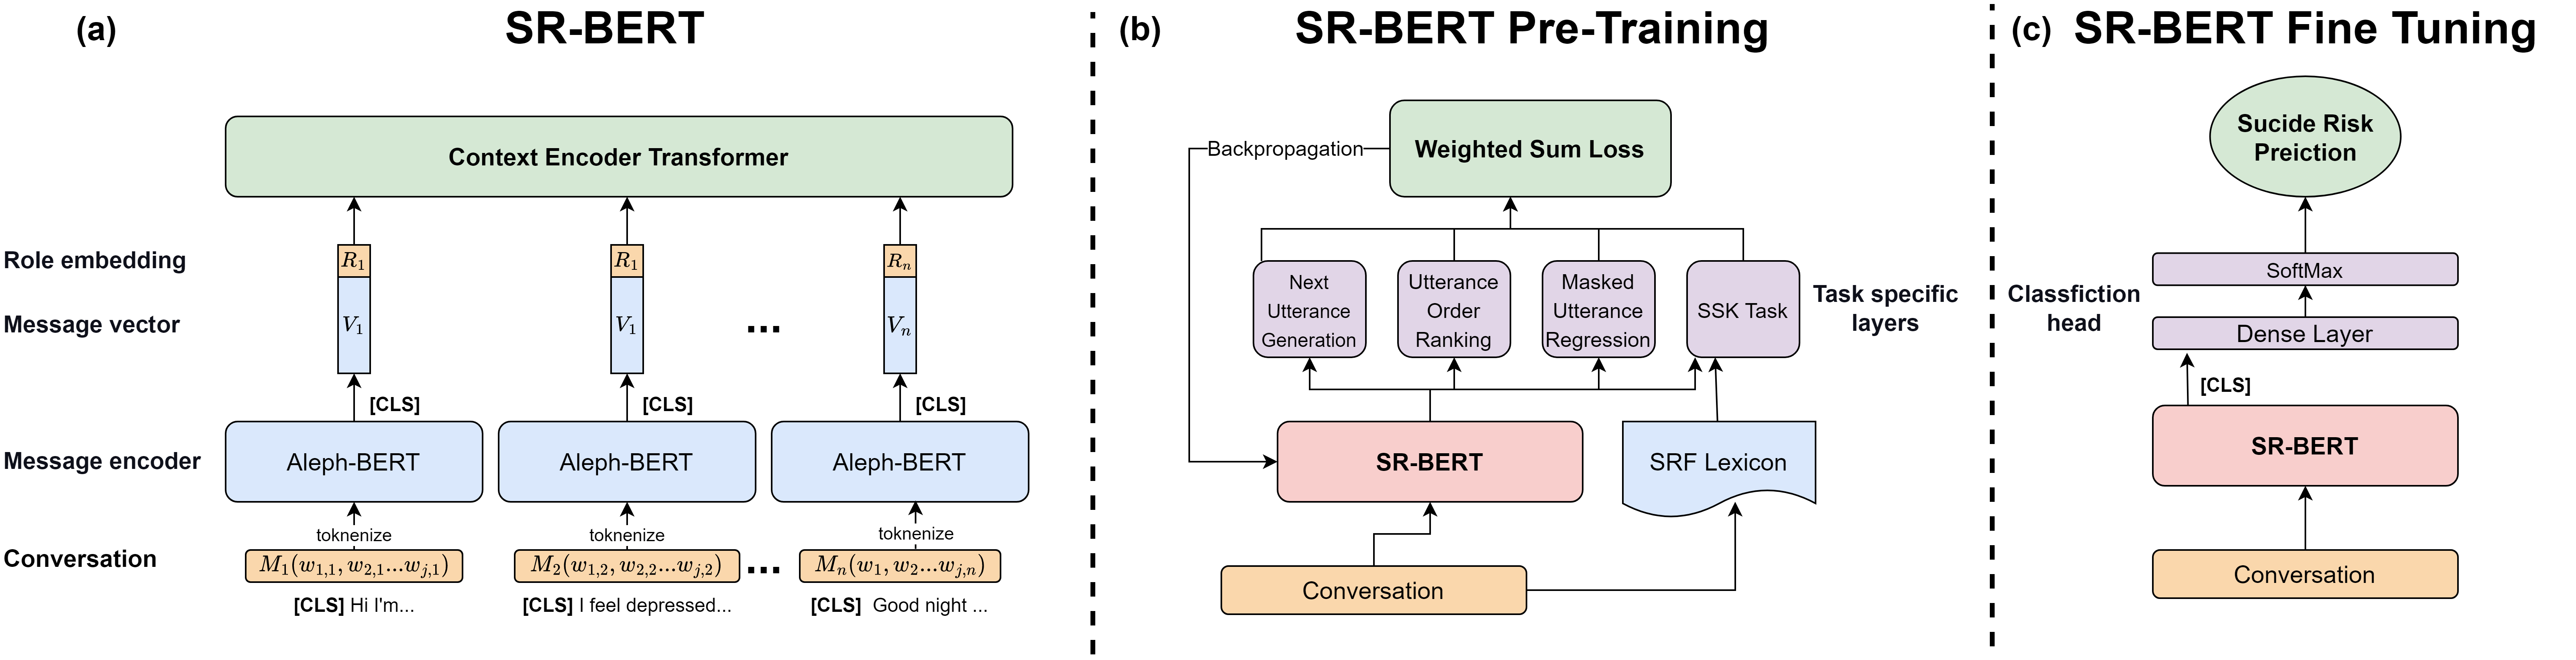
\includegraphics[width=2.2\columnwidth]{figures/ModelArchitecture.png}
\caption{Model architecture. (a) SR-BERT base architecture, encoding conversation and speaker roles.
(b) Pre-training procedure on 4 self-supervised tasks including psychological knowledge learning using the SRF lexicon.
(c) Fine-tuning procedure learning to predict Suicide Risk (SR)}

\label{fig:Architecture}

\end{figure*}

Our main contribution is
SR-BERT,  a two-layer hierarchical language model that  extends the generic DialogBERT~\cite{gu2021dialogbert} to reason about  conversation structure in suicide risk prediction settings and harness psychological domain knowledge.
The SR-BERT architecture is shown in \autoref{fig:Architecture}(a).
% We extended DialogBERT~\cite{gu2021dialogbert} with Hebrew language support and representation of  speaker roles (help seeker vs. counselor) into the dialogue model.
% The resulting model,

% \kg{revise to be clear about how you captured two aspects of conversation structure - speaker role and turn taking.}
% \di{the model captures this in implicit way, trough the combination of role representation and the related pre-training tasks.}

The architecture is composed of two part: A transformer based layer performing message encoding, and on top of it an additional transformer layer, which captures conversation structure, named  Context Encoder Transformer.

The base layer uses the AlephBERT~\cite{seker2022alephbert} pre-trained language model to encode each message in the dialogue to a vector. The received message encoding is then combined with speaker role representation (help-seeker vs. counselor) to capture important conversation aspects such as turn-taking. The Context Encoder Transformer is a transformer based encoder applied at the message level (instead of the single token level) which transforms the series of message vectors into a context-sensitive repression of the conversation.  The Context Encoder Transformer included 12 attention layers, and 12 hidden layers, each with a vector size of 780. The hidden layer size is 780 rather than 768 in AlephBert to account for the additional speaker role encoding.

The hierarchical structure of the architecture enables the model to capture multiple messages including turn exchanges and speaker roles. Furthermore, it enable the encoding of each message independently, thus avoiding the need to truncate conversations (due to  AlephBert's 512 token limit) as in past work.

% To obtain a the representation of the conversation we employ a hi
% % Finally, the the entire conversation was encoded in the Context Encoder Transformer component.
% %This layer has the same hyper-parameter settings as AlephBERT, with the exception of the hidden layer size, which is of 780 length rather than 768 to account for including the speaker role encoding. Overall,
% The structure
%\kg{The below is out of place in a paragraph that describes SR-BERT, suggest to remove. You   say later in the discussion that Amir was constrained. The example should only be used if it exists in the dataset.} \di{ I think this is a strong case why to use the hierarchical  model, where do you suggest to move it?  }

%One characteristic of our domain is that conversations are rather long, with a mean number of tokens of $617$, which exceeds the $512$ token limit of Bert and AlephBERT. To circumvent this issue, earlier efforts~\cite{amir} abbreviated the text and focused solely on help-seeker messages. Such an  approach might cause the model to misinterpret the text and overlook important exchanges between help-seeker and counselor, which are crucial in dialogue-based communication. For example, a counselor may ask the help-seeker whether they feel strongly depressed or suicidal, to which and help seeker might simply reply with ``yes''. Cutting the counselor question out will deprive the model from a key exchange that may indicate SR. The hierarchical architecture can encode the entire dialogue thus bypassing such crucial barriers all together.


\subsection{Pre-training with  Self Supervised Knowledge}
In this section we describe the use of several pre-training tasks for adapting SR-BERT to conversation structure of online counseling, including a  new pre-training task for   incorporating the SRF lexicon. This procedure uses the entire Sahar dataset, and is shown in \autoref{fig:Architecture} (b).
%The first step  the  Sahar conversations in the SRF lexicon space, while the second space is a self-supervised
%pre-training task
%for incorporating the SRF psychological lexicon into SR-BERT.
%that used the entire Sahar dataset.
%and the SRF psychological lexicon, as presented in \autoref{fig:Architecture} (b).
%SR-BERT was pre-trained with four self-supervised tasks to capture (while considering speaker roles) and
%psychological knowledge semantics.

%Each section of the conversation is as follows. Let $i$ represent a particular message in the conversation that will be referred to as the response, and all preceding messages in the conversation will be referred to as context. $i$ will increase until it reaches the length of the conversion. The response pairs will be used throughout the pre-training process in this context.
%The term ‘SR-BERT’ at each step refers to the model obtained by the previous step.
%We now describe the different pre-traning tasks in turn.

%\subsubsection{Self-Supervised Knowledge (SSK)}
% In this pre-training task we use the model for SR detection with  conversations represented  over the SRF space.
%, may encourage it to focus on terms and representations that domain experts marked as key for identifying suicide risk.
%We hypothesis (\textbf{some work has shown that multi task learning can help downstream task, but not quite the same type of task, can I cite them?  }) that incorporating distilled domain information relevant to a downstream task as part of the pretraining step can guide model learning in a more focused direction and improve the model's downstream performance. In our example, we believed that the suicide risk factors are frequent in the text and can indicate whether or not the help seeker has Suicidal tendencies. \textbf{(can I say that? can I say that we will test this hypnosis later in the study?)} . Therefor we want to encourage the model to pay attention and reflect in the conversation embedding terms that domain experts believe are important for predicting suicide risk.

% \kg{The below is an important par that needs more expansion. There is an issue with using the term 'model', when actually you use a a version of it without the pretraining or fine tuning. See Amir's solution about explaining the model. }
%\kg{who is the psyc team? can be in the intro or SRF section.}
%As hypothesized by the psychology team,suicide risk factors may be prevalent in the text and can indicate whether the help-seeker is exhibiting suicide risk. As such, training SR-BERT with domain expert knowledge may hold strong SR prediction value.

The first step in this process is to represent  conversations as a $25$ dimension vector representing the different categories in the lexicon.
For a given conversation, the value at index  $k$ is the number of sentences in the conversation with at least one occurrence in the \(k\)th lexicon category.


% For a given message, the value at index  $k$ is $1$ if the message includes any sentence from this lexicon category, and $0$ otherwise. For a group of messages, we sum up the vectors of each message in the group. This
%equal to the number of categories in the SRF lexicon. The vector represents the categories,  from which sentences appeared  in the message.
%For a given conversation, the value at index  $k$ is the number of utterances in the conversation with at least one occurrence in the lexicon category.

We also considered a  reduced 5-dimension representation of conversations on the SRF lexicon space.  To this end we selected the  top categories using XGBoost feature selection~\cite{chen2016xgboost} on the SR prediction task of entire conversations.
We identified the top 5 categories as ``self perceived burdensomeness'', ``previous suicide attempt'', ``loss of hope'' ``self injury'' and ``suicidal thinking''.  The 5-dimension representation outperformed the 25-dimension representation on the validation set, leading us to use  this representation in the subsequent pre-training phase.


% We now present the Self Supervised Knowledge (SSK) task, a self supervised pre-training task based on domain knowledge. The training goal is to predict a conversation subset's encoding in the SRF lexical space while a randomly selected message is masked.
% Given  a conversation subset, we randomly choose a single message in that conversation and either mask it (with $80\%$ probability) - replacing it with `[CLS,MASK,SEP]'', or leave it as is (with $20\%$ probability). SR-BERT is then applied to obtain the conversation subset's vector representation (using the [CLS] representation). Then, a fully connected layer with an output size equal to the domain knowledge embedding layer receives this vector representation and attempts to predict the original SRF representation vector. The loss is obtained by calculating the mean squared error (MSE) between the original and predicted vectors. This process is repeated for all conversations subsets in the dataset.

%mask with a

The second step, called   the Self Supervised Knowledge task, applies a new pre-training task  for predicting  Sahar conversations in the SRF representation space.
%We mask an utterance in a given conversation
For  a given  prefix of a conversation, we  mask a message in this subset  with a fixed probability of 80\%.
We then use SR-BERT to predict the conversation subset's representation in the SRF space using a fully connected layer.
%Given  a conversation subset, we randomly choose a single utterance  and either mask it (with $80\%$ probability) - replacing it with `[CLS,MASK,SEP]'', or leave it as is (with $20\%$ probability).
%SR-BERT is then applied to obtain the conversation subset's vector representation (using the [CLS] representation).
%Then, a fully connected layer with an output size equal to the domain knowledge embedding layer receives this vector representation and attempts to predict the original SRF representation vector.
The loss is obtained by calculating the mean squared error (MSE)
between the original subset representation and the predicted (masked) representation in the SRF space.
This process is repeated for increasing size of conversation prefixes, to simulate conversations of varying sizes.

%Pre-training was performed on increasing lengths of conversation subsets  to simulate varying lengths of conversations.

% The training goal is to predict a conversation's encoding in the SRF lexical space while some randomly selected messages are masked. The training task uses the SR-BERT conversation embedding that was generated and connects it to a fully connected layer with an output size equal to the domain knowledge embedding. The loss is calculated using the mean squared error (MSE) between the predicted encoding and the actual SRF lexicon-based encoding.
%In order to capture the discourse-level coherence in dialog contexts, we propose two novel objectives inspired by BERT in addition to the conventional objective of response generation, i.e., maximizing the log probabilities of decoded words. Following three subsections describe the objectives in turn.

In addition to the SSK task, we implemented  the  three pre-training tasks defined by DialogBERT\cite{gu2021dialogbert} for capturing several aspects of the conversation structure: message-level semantics, conversation structure, and underlying dialogue sequential order. We describe them briefly here and refer the reader to the full paper for more details.


\begin{itemize}
    \item \textbf{Next Utterance Generation}  The goal of this task is to generate the next message in the conversation when the previous messages are given. The task tries to minimize the cross-entropy loss between the predicted words and the original words of the next message.

    \item \textbf{Masked Utterance Regression}  The goal of this task is to predict a randomly masked message in a conversation from its context. The loss is obtained by calculating the MSE between the original and the predicted message vectors.

    \item \textbf{Distributed Order Ranking Network} This task predicts the order index of each message from a shuffled order of a conversation. The task tries to minimize the KL divergence between the predicted order and the true order.
\end{itemize}
%The
%These allow us to

%pre-training tasks were implemented to capture the conversational structure of each session:

% \cite{gu2021dialogbert} and are described here briefly. We refer the reader to the full paper for more details.
% \kg{you don't even need to describe them briefly, you can say you implemented the following pretraining tasks from dialogBERT for masked utterance, etc...}

% \subsubsection {Masked Utterance Regression} a self supervised task inspired by the original Masked Language Model (MLM) task of the  BERT model \cite{devlin2018bert}. Instead of randomly masking tokens from the input and having the model predict the masked input, this task randomly masks input messages while the model tries to reconstruct the masked message vector. The hierarchical model is first applied on the context of the message to obtain the message representation vector. Then, a fully connected layer receives the contextualized message vector and attempts to reconstruct the original message vector. The loss is obtained by calculating the MSE between the original and predicted message vectors.

% \subsubsection {Message Order Ranking} The goal of this task is to re-order randomly shuffled messages from the conversation into the original conversation order. This is done by an order prediction network - a dense network that takes as input the hidden states of the shuffled messages from the context encoder and calculates a score for each individual message.
% %The order prediction network computes the pairwise inner products between hidden states and then calculates the score for each utterance by averaging all its inner products with other utterances. Given these scores, we estimate the “rank-1”probability for each utterance with softmax.
% The goal is to minimize the KL divergence between the predicted order and the true order. Such learning embeds the significance of message ordering into the learnt language model as well as the roles of the speakers in the different ordered messages.
% %\di{I need some help to re write it in more of my words.}


% \subsubsection {Next Message Generation} The goal of this task is to generate the next message in the conversation when the previous messages (context) are given. First, A contextualized message vector from the context is created. A transformer decoder is then used predict distribution of probabilities for words in generated message. Each new word is predicted by using the contextualized message vector and the previously predicted words. The task tries to minimize the cross-entropy loss between the predicted words and the original words.
% The core assumption is that this learning task will help the model better represent the semantic dialog features of the conversation.
% %index over the vocabulary \di{I have difficulty explaining it without using formulae. In the paper, they just say predict words, and the formulae explain it in detail}

The calculated loss for the model propagation over the four self supervised tasks is the weighted sum of each loss function in the pre-training stage.
The AdamW optimizer is employed with a linear planned warm-up technique and an initial learning rate of 5e-5.
Additionally, we use an adaptive learning-rate scheduler with 0.01 weight decay, 15,000 warm-up steps, and a batch size of 32. The model is trained for 20 epochs.
All experiments are conducted on a GeForce RTX 3090 GPU using the the PyTorch package.

\subsection{Fine-tuning}

In the fine-tuning step \autoref{fig:Architecture}(c), SR-BERT is adapted for the  suicide risk prediction task using a standard approach \cite{sunHowFineTuneBERT2020}. %trained to predict Suicide Risk for each conversation
To this end we add a binary classification head to SR-BERT. The classification head consists of a dense layer with an output size of 2 and a softmax activation function.
%The [CLS] obtained from passing the conversation through the SR-BERT model serves as the classification head input.
By maximizing the log-likelihood of the actual label, we fine-tune the Context Encoder Transformer and the classification head.
We employ the AdamW optimizer with a linear planned warm-up technique and an initial learning rate of 2e-5. Additionally, we use an adaptive learning-rate scheduler with 0.01 weight decay, and a batch size of 16. The model is trained for 10 epochs.



\begin{table*}[]
\centering
\caption{SR prediction results of compared models. Bold highlights highest value.}
\scalebox{1.2}{
\begin{tabular}{rccccc}

\hline
\multicolumn{1}{c}{Model} &
  \multicolumn{1}{l}{Recall {[}\%{]}} &
  \multicolumn{1}{l}{Precision {[}\%{]}} &
  ROC-AUC {[}\%{]} &
  F2 {[}\%{]} &
  F1 {[}\%{]} \\ \hline
Doc2Vec+XGBoost                  & $31.3$          & $69.2$          & $64.7$         & $35.1$          & $43.1$          \\
Explicit lexicon+XGBoost         & $49.2$          & $67.1$          & $76.9$          & $52.3$          & $57.7$          \\
SRF lexicon + XGBoost & $55.1$ & $67.2$ & $76.5$ & $57.1$ & $60.0$ \\
Ensemble SI-BERT & $60.4$          & $\mathbf{70.9}$ & $91.3$          & $62.3$          & $65.3$          \\
SR-BERT w.o. SSK                 & $72.9$          & $68.4$          & $\mathbf{92.1}$ & $71.9$          & $70.6$          \\
SR-BERT w. SSK                   & $\mathbf{78.3}$ & $68.9$          & $\mathbf{92.1}$ & $\mathbf{76.2}$ & $\mathbf{73.3}$ \\ \hline


\end{tabular}
\label{tab:EntireRes}
}
\end{table*}


\section{Empirical Methodology}

We randomly  split   the labeled Sahar dataset  to a train ($70\%$) validation ($15\%$) and test ($15\%$) sets. These data sets were used throughout the experiments described in the following section. The validation set was used for training model hyper parameters.
%Pre-traning was performed using the entire Sahar dataset (including labeled and unlabeled conversations).

%\subsection{Evaluation Metrics}
%\label{sec:Evaluation Metrics}
We follow prior work in evaluating model performance using ROC-AUC which is widely employed in suicide detection research~\cite{bernert2020artificial}. Additionally, we report on the F2-score~\cite{sokolova2006beyond} for predicting the positive SR label. This measure concentrates on reducing false negatives (rather than false positives) and is thus well suited for SR detection where missing a positive class has life threatening implications.
%We note that ROC-AUC considers sensitivity and specificity equally, while the F2-measure is a weighted sum that favours recall over precision.


% which is incorrect for our case study. In our instance, the tolerance for false negatives is substantially smaller than for false positives, thus we will use the F2 measure to evaluate our model. The F2-measure concentrates on reducing false negatives rather than false positives and is derived using a weighted sum in which recall is weighted twice as much as precision. The reported F2 score is the score received the positive class that represent GSR positive conversation and is the minority class.

%\subsection{Baseline Models}

We compare SR-BERT with SSK to the following baseline models:

\paragraph{SR-BERT w.o. SSK} This  model omits the SSK pre-training task from SR-BERT w. SSK. Apart from the SSK pre-training task this model is identical to SR-BERT w. SSK. including the hierarchical structure and pre-training on the other 3 tasks.

 \paragraph{Ensemble SI-BERT~\cite{amir}}
 This is a non-hierarchical Hebrew language model
 that represents the state of the art for SR detection. It was trained on the same dataset from the Sahar organization.  To bypass BERT's constraint of 512 tokens, Ensemble SI-BERT only utilized the help seeker text and truncated text greater than 512 tokens. %that was traned and fine-tuned using the same dataset as AlpehBERT.
%This model only considered the help seeker utterances in a conversation, truncating conversations to a maximal size of 512 tokens.
We re-implemented this model with the code and parameters provided by the authors and run it on the dataset provided for this research.
 This is the reported state of the art for this domain in the Hebrew language.


\subsubsection{SRF based lexicon + XGBoost}
An XGBoost~\cite{chen2016xgboost} classifier based on  an encoding of conversations over the Suicide Risk Factor (SRF) lexicon. We note that XGBoost outperformed Random Forest and Logistic Regression as the classifier for this baseline (and for the next two baselines)

\begin{figure}[t]
\centering
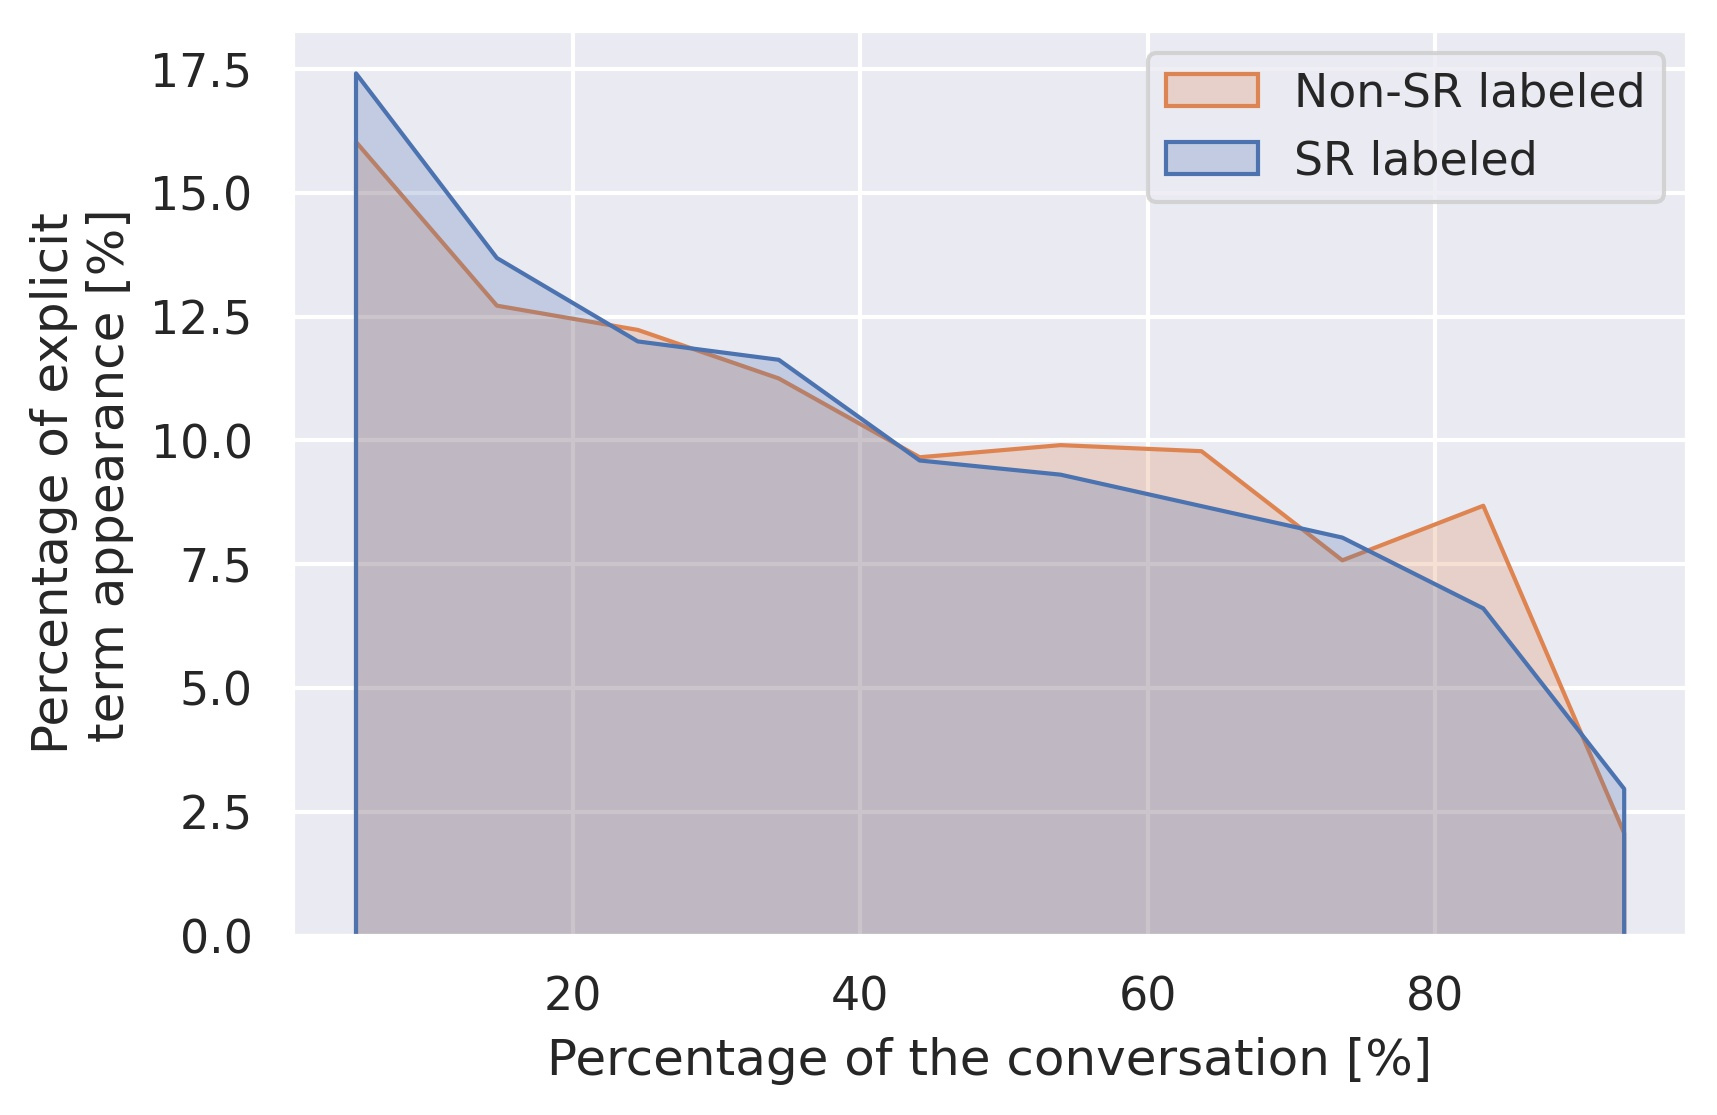
\includegraphics[width=1.05\columnwidth]{figures/explicit_mention.jpg}
\caption{Distribution of explicit appearance of suicidal terms in  the labeled Sahar dataset. Dark colors represent overlapping values.}
\label{fig:ExplictDis}
\end{figure}

  \subsubsection{Explicit based lexicon + XGBoost}
We used an XGBoost classifier that was based on an encoding  of conversations over the explicit suicide related terms proposed by ~\citet{amir}. This  list  includes 67 terms such as ``commit suicide'', ``cut wrists'', ``wish to die'' etc.
We note that explicit terms carry very weak signal for SR detection.  This is apparent in
\autoref{fig:ExplictDis} which presents the distributions of explicit terms throughout the session for SR and non-SR labeled  conversations. As seen in the figure, the distributions over both classes are similar.
Consider for example one of the sessions which includes the statement ``I am having strong stomach aches since yesterday, I want to die.''. This session includes a term from the Explicit lexicon while it is not an SR positive session.

%  \subsubsection{Explicit-Lexicon} trained XgBoost classifier that receive counting vector based on Lexicon based on explicit mentions described in \autoref{subsec:Explicit Lexicon}

\subsubsection{Doc2Vec + XGBoost}
%Due to the lack of a benchmark for SR detection in online consulting services, we choose to compare our approach to a non-Transformer-based solution, Doc2Vec.
An XGBoost classifier based on an encoding of each conversation to a 300-dimensional space using the Doc2Vec representation\cite{doc2vec} .

\section{Results}
We first present the performance of the SR-BERT model in predicting SR on labeled conversations compared to the proposed baselines.
Results are then reported for early SR detection, when increasing percentages of conversation information are available. Finally we look at the contribution of the SSK pre-training task for SR detection in the case of conversations where no explicit suicide related terms are present.
%We conducted several sets of experiments to evaluate the SR-BERT model and specifically, the contribution of the SSK pretraining task to predicting SR.


% In this section, we will conduct four sets of experiments to thoroughly examine our SR-BERT model and the implication of training with SSK task.

% The first exam will cover whole sessions, while the second will concentrate on early detection. The final two tests will be run on increasingly difficult data sets.


\begin{figure}[]
\centering
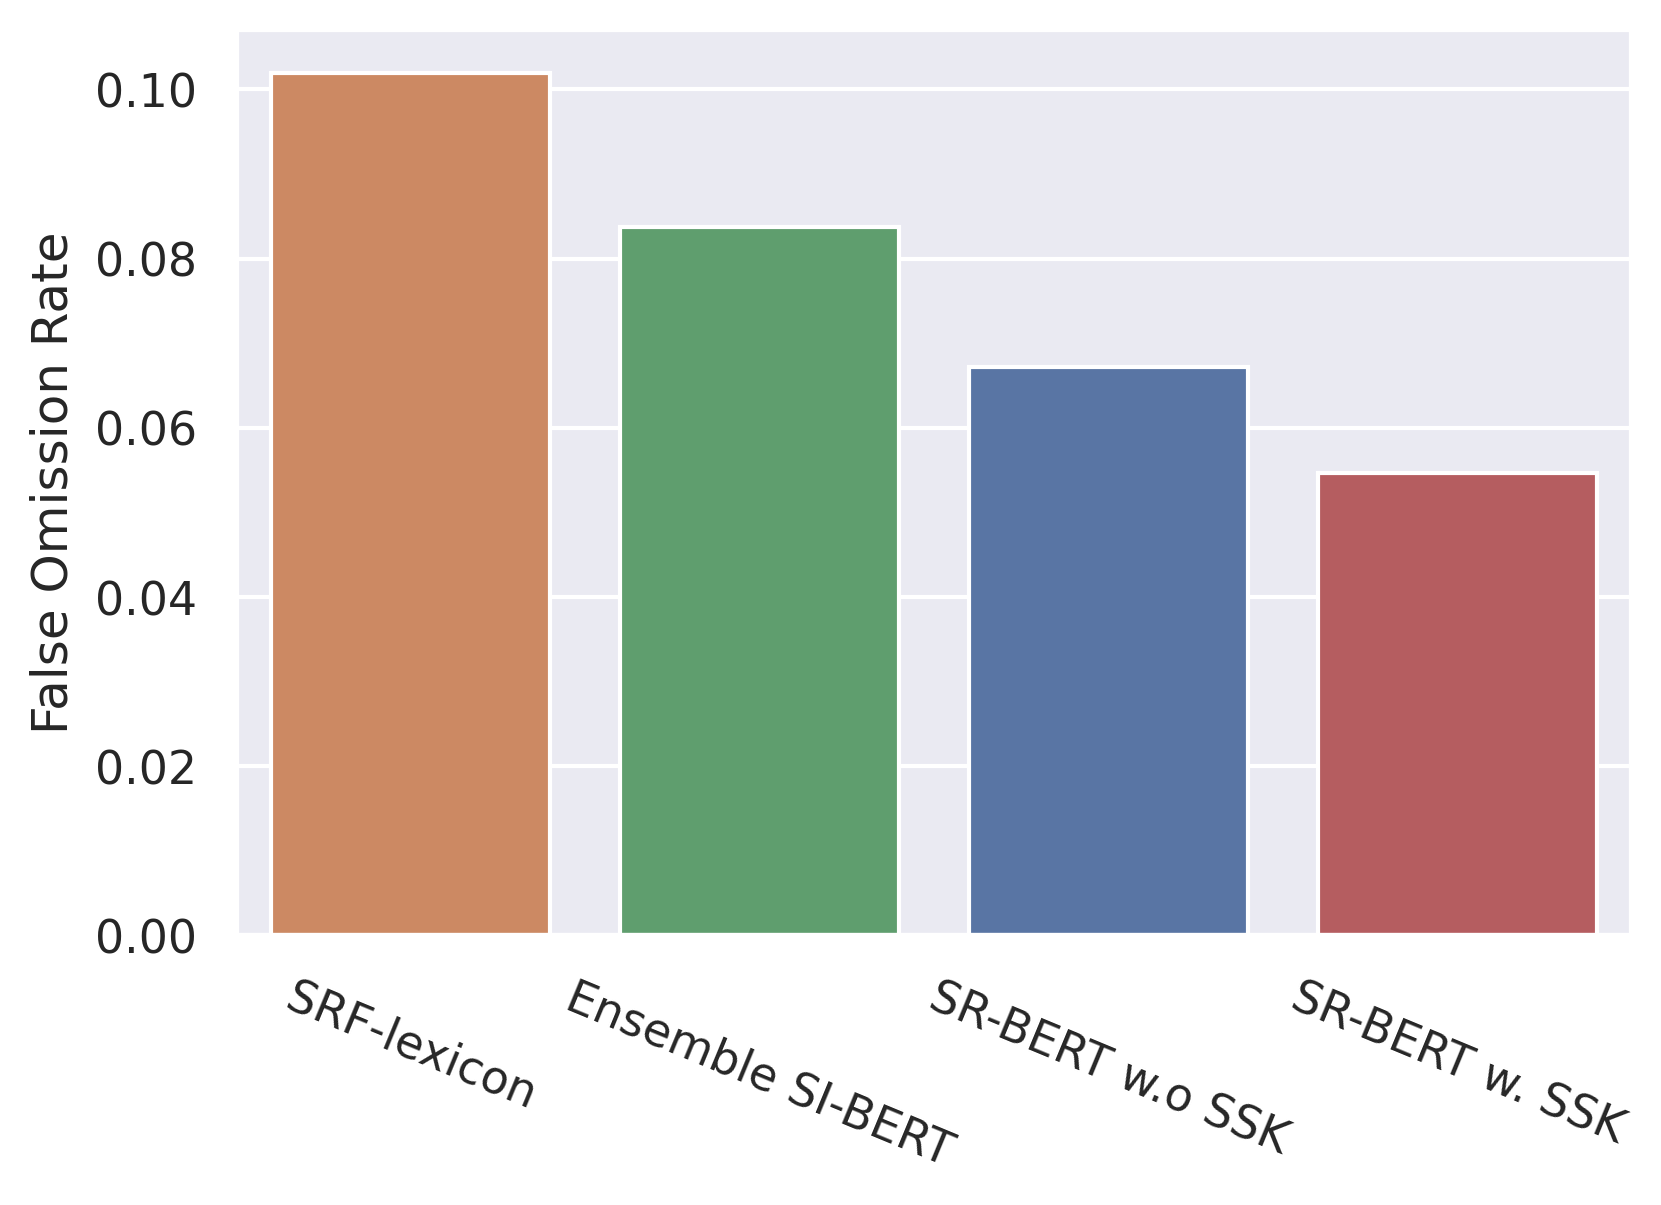
\includegraphics[width=1.05\columnwidth]{figures/Omission_Rate.png}
\caption{False Omission Rate of different models.}
\label{fig:omission_rate}
\end{figure}


\subsection{SR Detection from Complete Conversation}

\autoref{tab:EntireRes} compares
the performance of the SR-BERT model to the baselines when predicting suicide risk from complete conversations.
As seen in the table, both SR-BERT-based models (with and without SSK pre-training) outperformed the Ensemble SI-BERT model in terms of recall, F1, F2, and ROC-AUC metrics. Most notable improvement was in the recall metric where SR-BERT w.o. SSK achieved a $12.5\%$ improvement over the Ensemble SI-BERT model, which led to a $9.6\%$ improvement in the F2 metric. Moreover, the additional SSK pre-training improved on the SR-BERT w.o. SSK results for all metrics except the ROC-AUC score, where it hasn't change.
  %although in less significant amount.
Ensemble SI-BERT achieved the highest precision, which was slightly better than SR-BERT w. SSK. It exhibited a substantially lower recall score, which correlates to lower F1 and F2 values.

The SRF lexicon + XGBoost based classifier was better than the Explicit lexicon + XGBoost classifier in all measures apart from ROC-AUC.
We also note that the BERT based models outperformed the none BERT models on all tested metrics.

We used the  McNemar paired test for labeling disagreements~\cite{gllick} to compare between SR-BERT w. SSK and the two models SR-BERT w.o SSK and Ensemble SI-BERT. Statistical significance with $p < 0.05$ was demonstrated for SR-BERT w. SSK vs SR-BERT w.o. SSK and for SR-BERT w. SSK vs Ensemble SI-BERT.

%Statistical significance (with the, ) between Ensemble SI-BERT vs SR-BERT w.o. SSK, .
%he lexicons and the Doc2Vec model were both outperformed by all the BERT-based language models.

%Since, in general, language models based on Transformers perform better than more conventional baselines, notably in morphological rich languages like Hebrew.
Overall SR-BERT w. SSK achieved a substantial improvement in recall and F2 compared the Ensemble SI-BRET of $17.9\%$ and $13.9\%$  respectively, with only a slight decrease in precision performance. This is critical in the suicide risk detection realm where recall is key to identifying help-seekers at risk and enable targeted support.
%because, as discussed in \autoref{sec:Evaluation Metrics}, we aim to minimize our models' false negatives. We may compute the false omission rate metric,

To further analyze this issue,  \autoref{fig:omission_rate} compares the False Omission Rate for the different models, which is the fraction of false negative instances out of the set of all predicted negative instances.
%
%instances with a negative SR label for which the genuine condition is positive, out of the e
As seen in the figure, the SR-BERT models without SSK was able to reduce the False Omission Rate relative to the Ensemble SI-BERT Model from 0.083 to 0.067, a $19.2\%$ improvement. Pre-training SR-BERT with the additional SSK task further reduced the False Omission Rate from  0.067 to 0.054, a total of $34\%$ reduction compared to Ensemble SI-BERT.

\subsection{Early SR Detection}

\label{ExplicitLex}
\begin{figure}[]
\centering
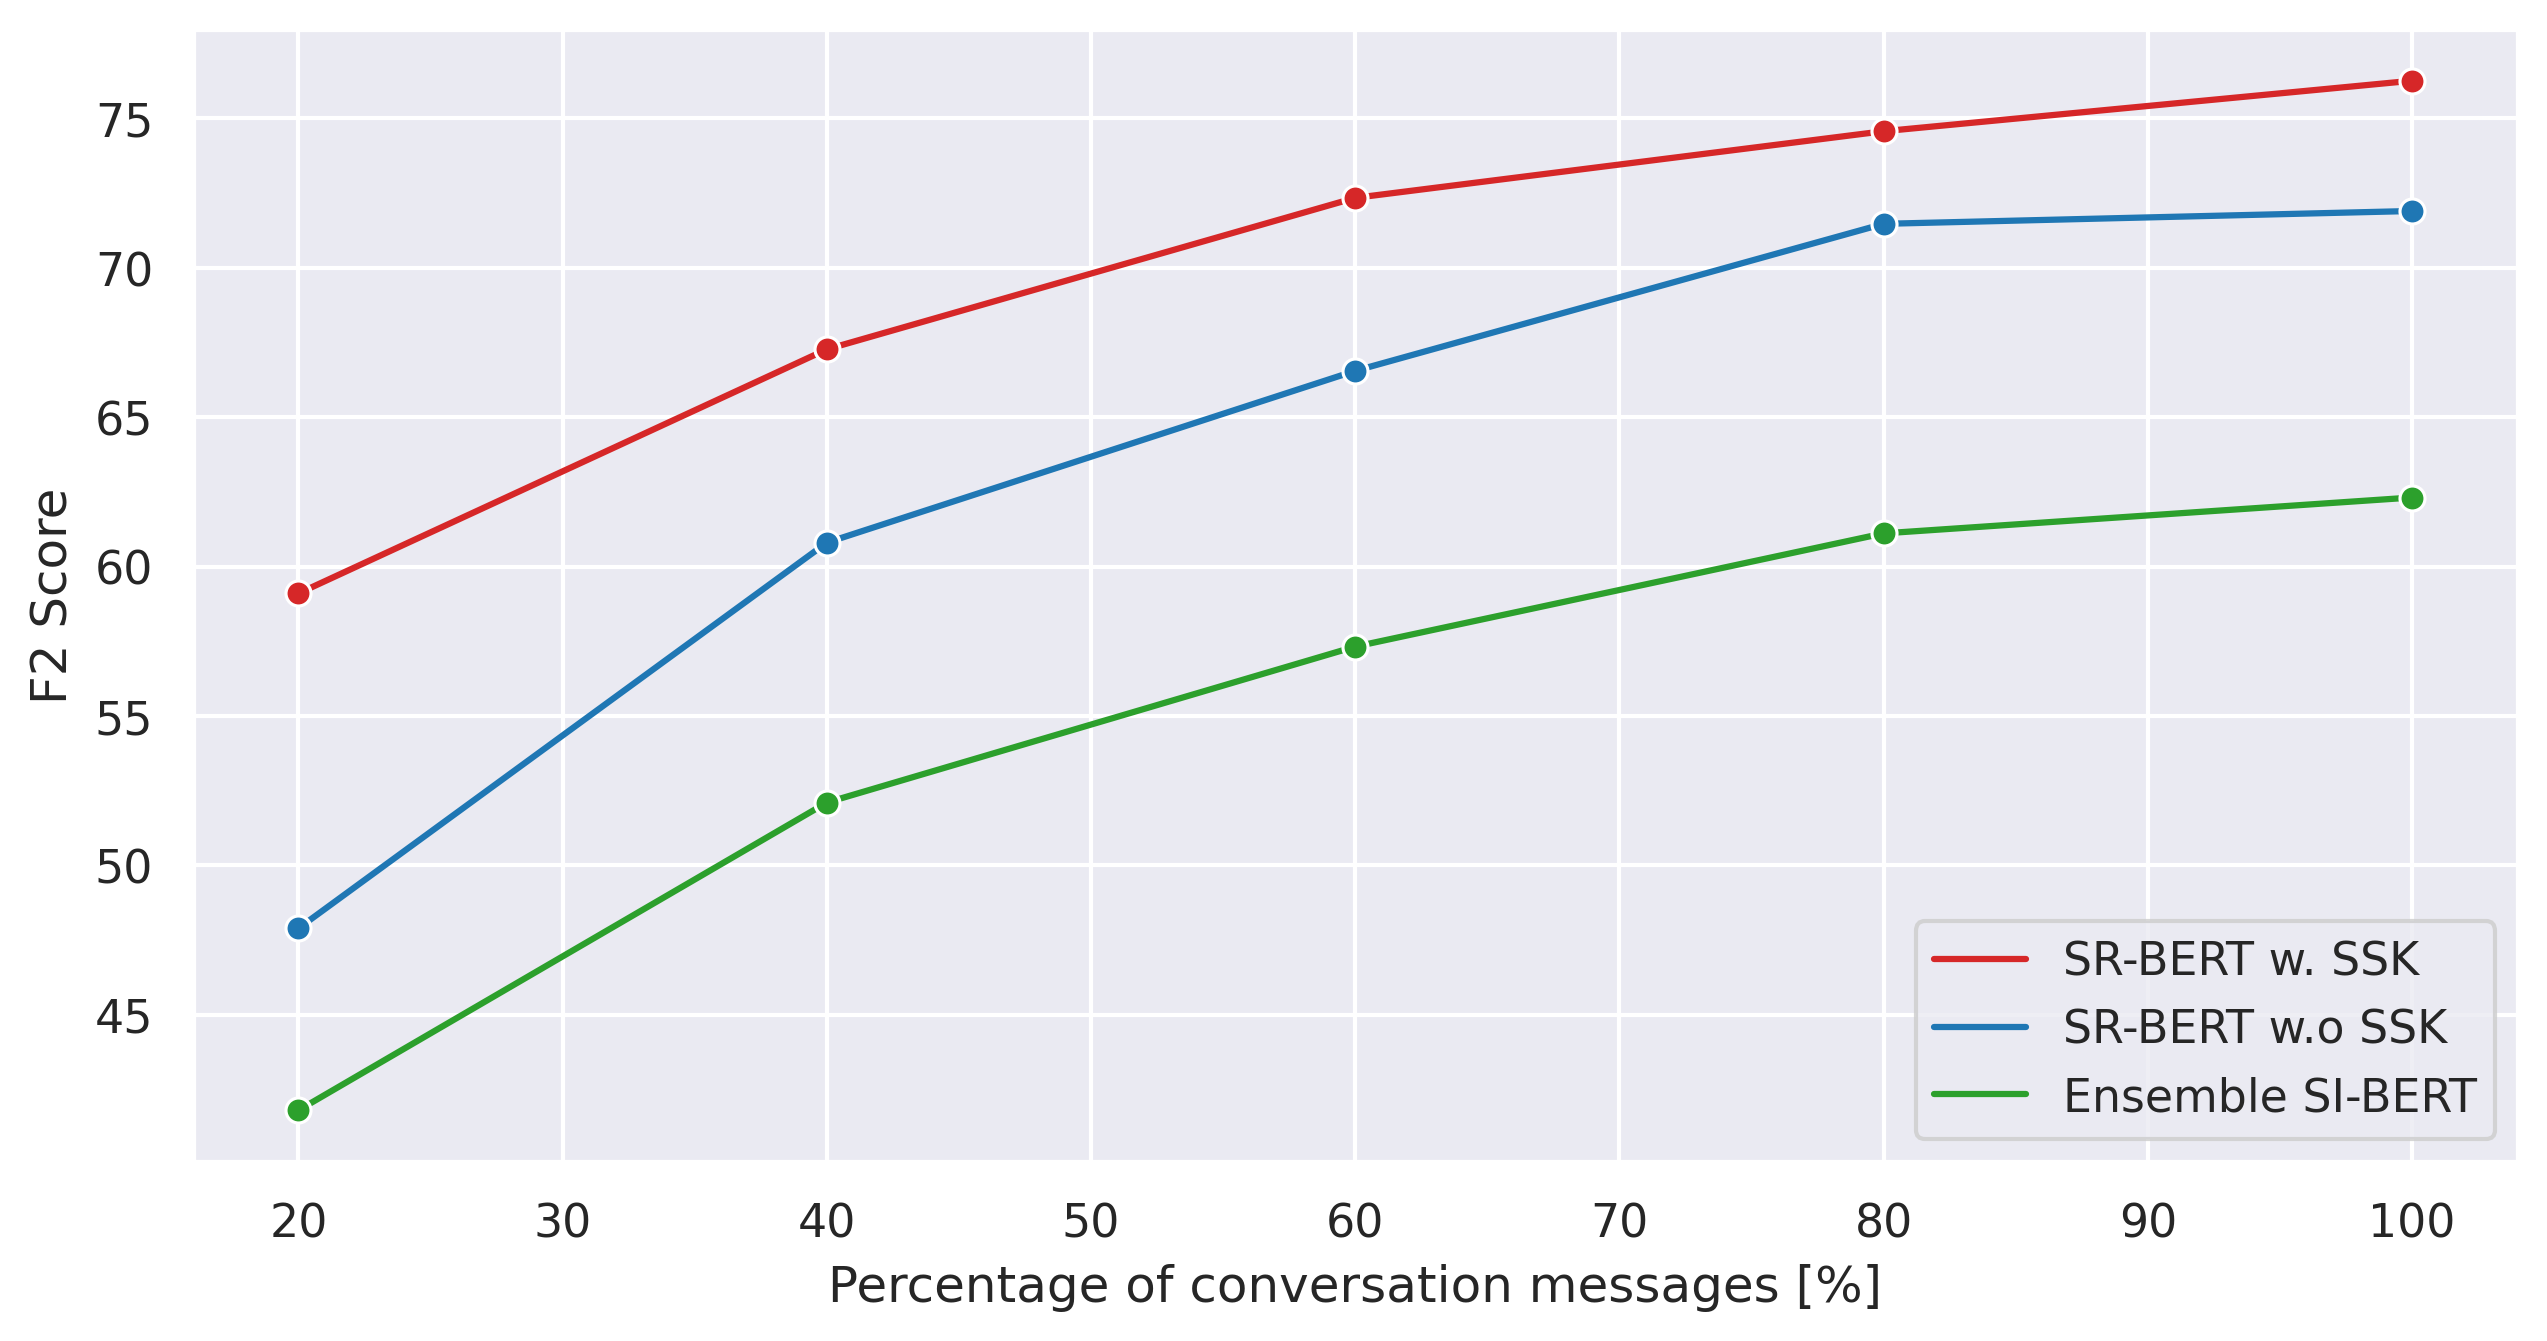
\includegraphics[width=1.04\columnwidth]{figures/normal_F2.png}
\caption{Classification results for early detection of top-performing SR detection approaches}
\label{fig:Early detection}
\end{figure}

Evaluating the  ability of SR-BERT to predict SR risk  from  partial sessions provides an indication of  its  performance in real time, when only part of the session is  available.
%which can potentially facilitate  deployment as a support tool for hot-line counsellors.
%lessens the workload for the volunteers, and can assist in identifying which help seekers have a greater suicide risk.
To this end, \autoref{fig:Early detection} compares the performance of the different models  after receiving the first  $\{20,40,60,80,100\}$ percent of messages in the session.
%As might be predicted,
As seen in the figure, the  performance of all models improved  as the sessions progressed.  However, SR-BERT w. SSK model consistently outperformed the other models, followed by SR-BERT w.o. SSK.
The difference in  performance   between SR-BERT with SSK and SR-BERT w.o. SSK was the largest at the beginning of the session and reduced as the sessions advanced.
This  may indicate the contribution of  SR-BERT w. SSK to identify risk variables from the lexicon in early stages of the dialogue when information is lacking.
%Kobi -  to the discussion. We theorize that this is a result of the model's capacity to identify   early suicide risk variables in the dialogue, which plays a greater role when information is lacking
In contrast, the  difference in performance  between SR-BERT w.o. SSK and the Ensemble SI-BERT model increases as sessions advance.
This could be due to the inability of Ensemble SI-BERT to  process the lengthy dialogue without having to truncate it, which may result in the loss of important information as sessions develop.
% Moreover, we notice the performance difference between SR-BERT w.SSK and SR-BERT w.o. SSK decreases as the sessions advance.
% This maybe is caused by the lack of information in the early part of the conversation, which causes the model to be more dependent on the knowledge gathered from the SSK task.
% \subsection{The Contribution of the SSK task}
% \begin{figure}[h]
% \centering
% 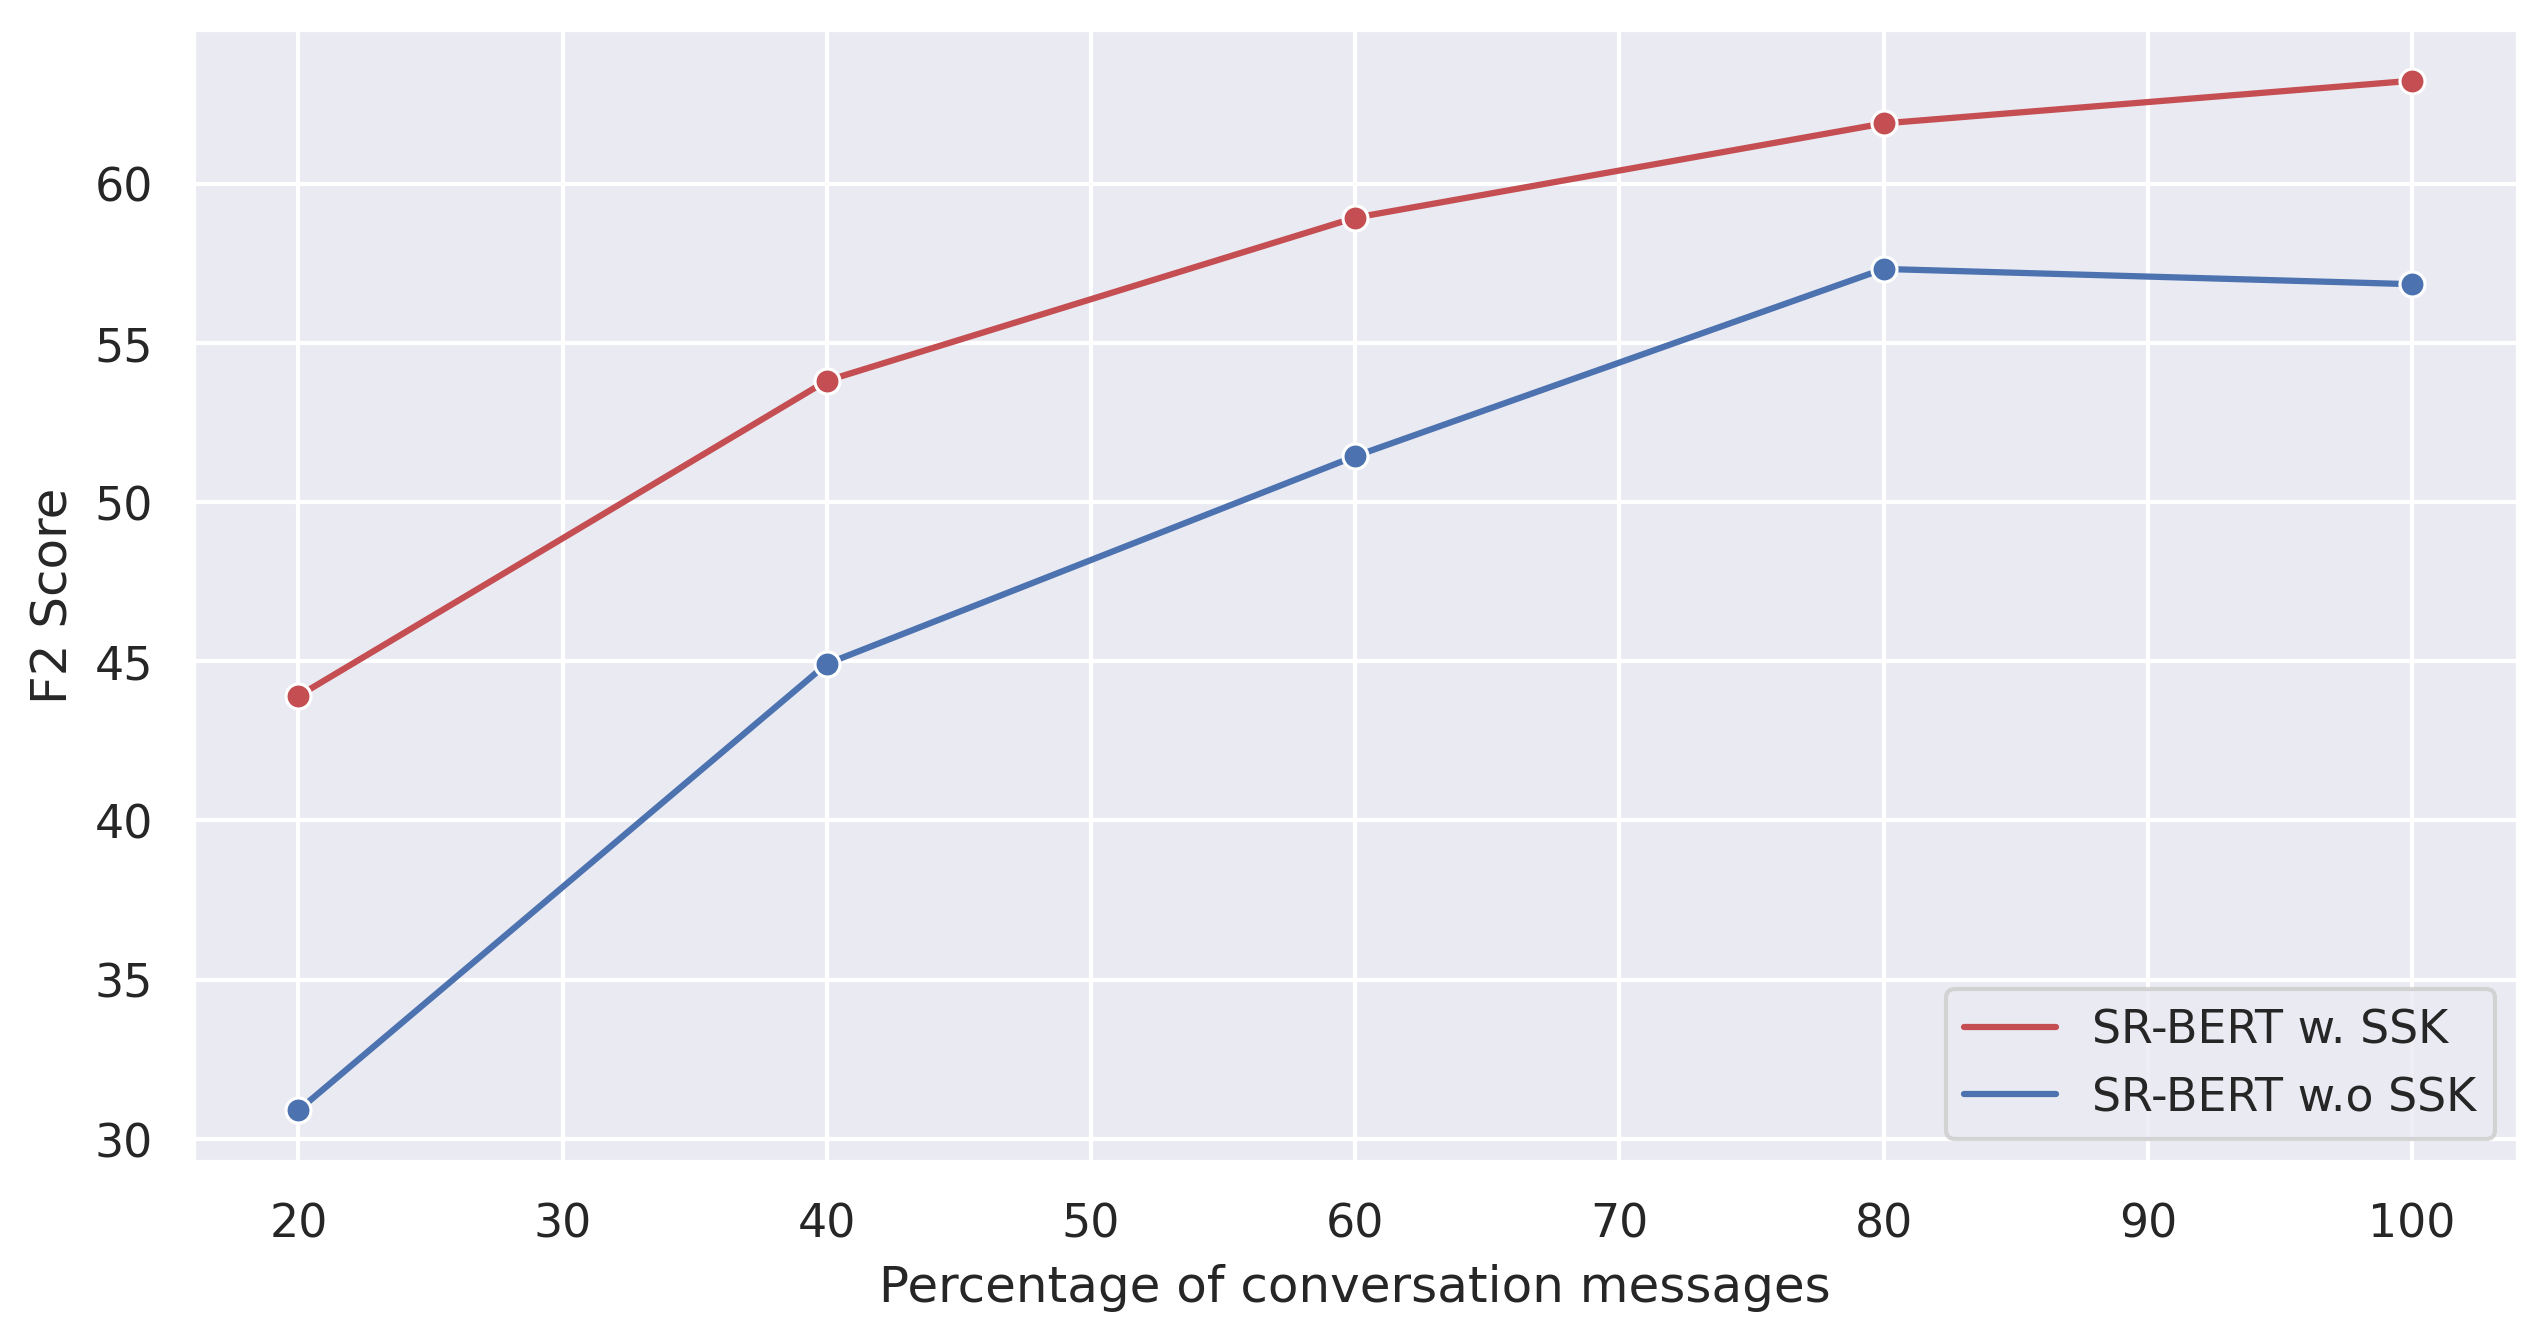
\includegraphics[width=1\columnwidth]{figures/explict_F2.png}
% \caption{Classification results for early detection on explicit-less-terms test benchmark.}
% \label{fig:explicit-less-terms}
% \end{figure}


\begin{figure}[h]
\centering
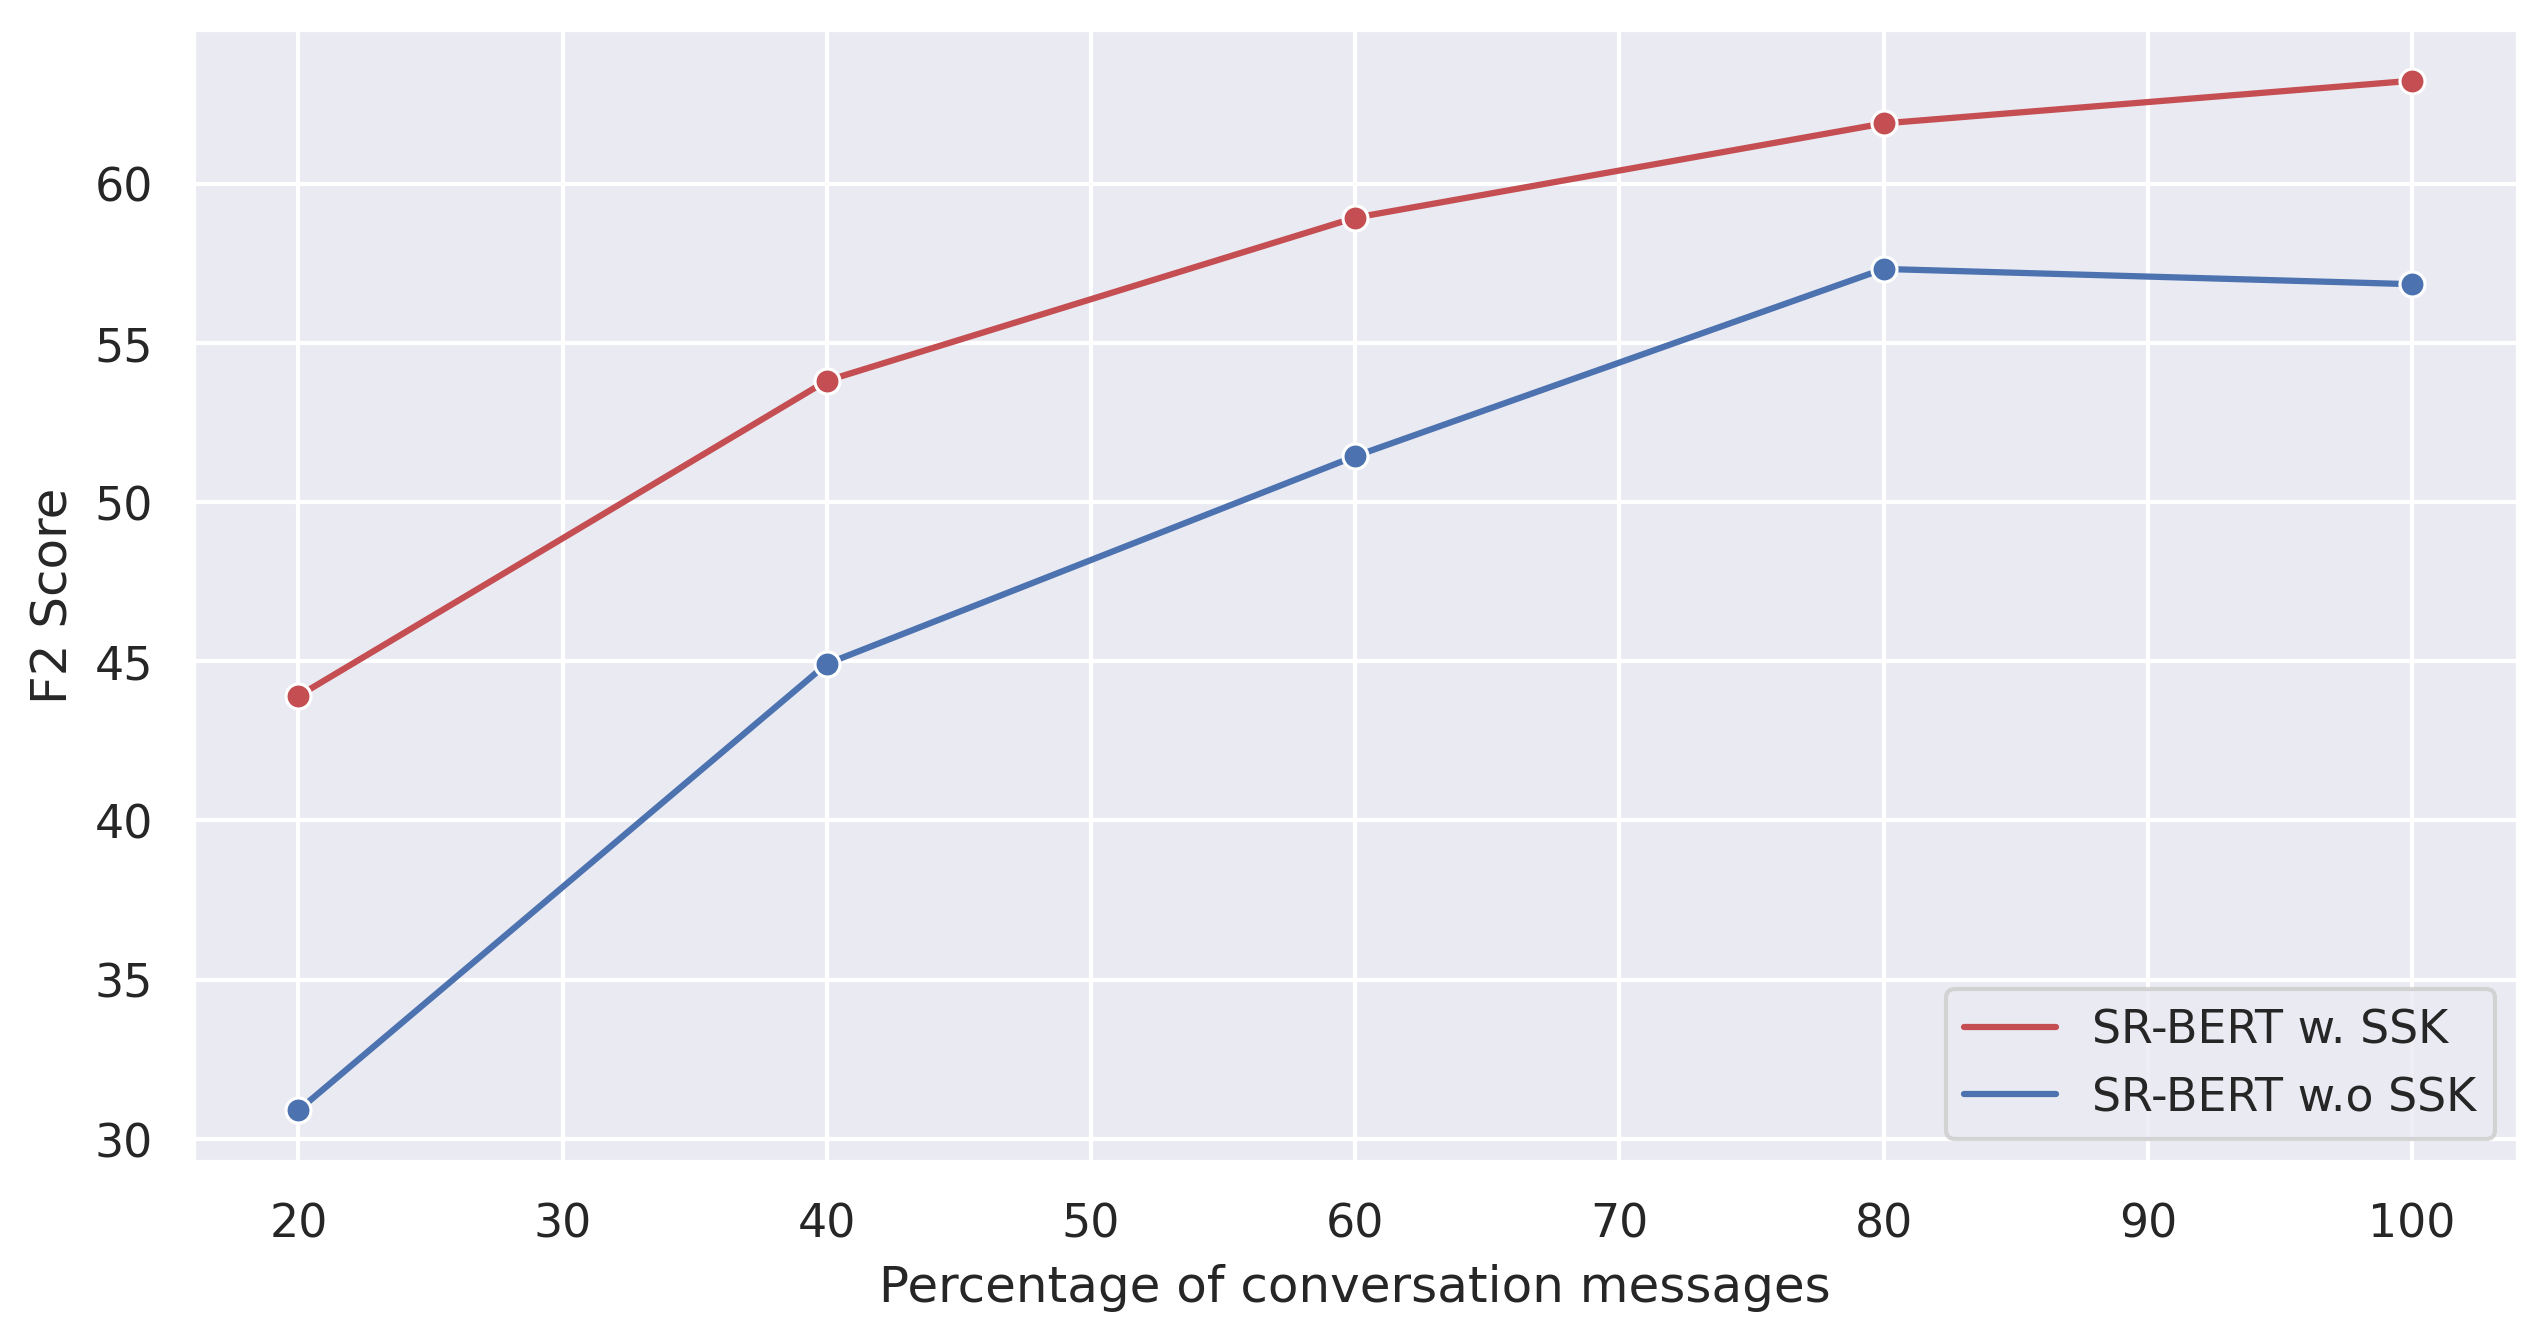
\includegraphics[width=1.04\columnwidth]{figures/explict_F2.png}
\caption{Classification results for early detection on explicit-less-terms benchmark.}
\label{fig:explicit-less-terms}
\end{figure}

\begin{figure}[h]
\centering
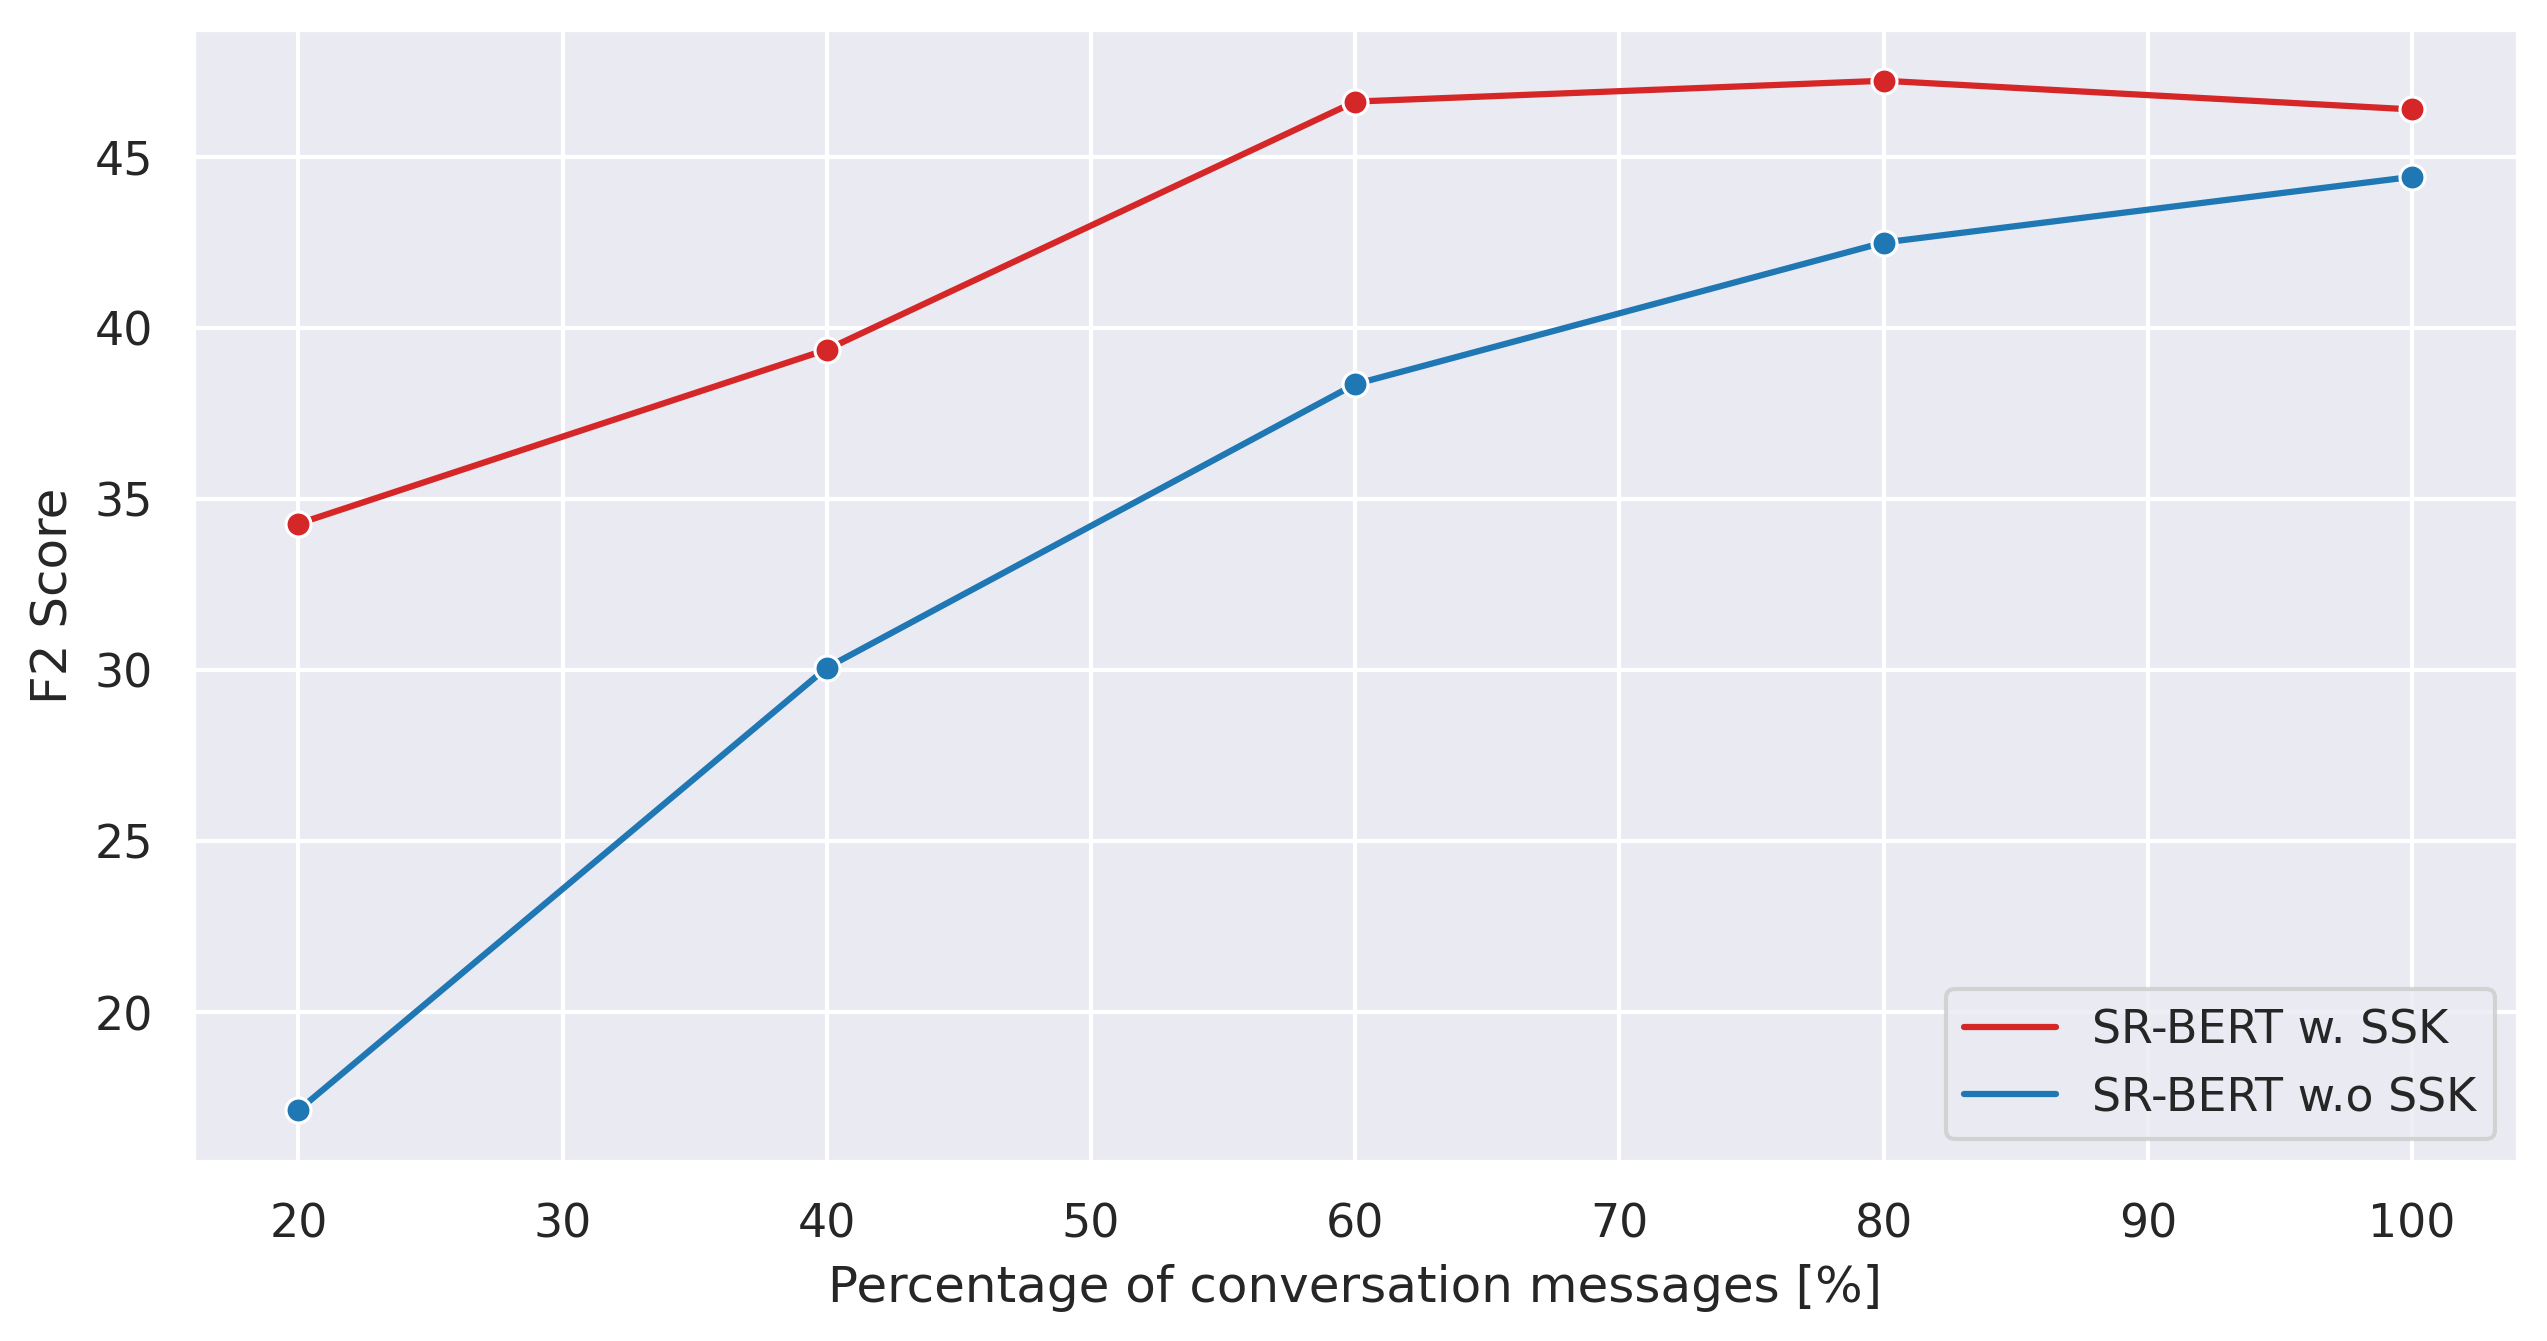
\includegraphics[width=1.04\columnwidth]{figures/explicit_conv_F2.png}
\caption{Classification results for early detection on explicit-less-conversations benchmark.}
\label{fig:explicit-less-conversations}
\end{figure}


To further assess the contribution of the SSK task, we compared the performance of the SR-BERT w. and w.o SSK on benchmark datasets that do not contain explicit mentions of suicide terms (from the Explicit based lexicon). Specifically, the ``explicit-less-terms`` benchmark dataset omits all explicit mentions of suicide terms from the testset, retaining the same number of messages.
The ``explicit-less-conversations'' benchmark dataset omits all conversations with any mention of a suicide term from the Explicit lexicon.
% This dataset has 1,268 conversations, 64 of which are labeled as SR positive conversations.

%We follow the methodology of \citet{caoLatentSuicideRisk2019} who evaluated a model for suicide risk detection in blog posts on a subset of instances
 %We created two subsets of tests to assess the capability of our model. The first, dubbed explicit-less-test, was built by removing all explicit mentions from all conversations, yielding the same size test set but with missing words.The other test set is called "Non-explicit-sub-test," and it is made up of a subset of the test set that contains no explicit mentions at all. The Non-explicit-subtest has 1268 conversations, 64 of which are labeled as GSR positive conversations.

The performance of SR-BERT with and without SSK pre-training  on the two benchmark datasets is presented in \autoref{fig:explicit-less-terms} and \autoref{fig:explicit-less-conversations}. As expected, the overall performance of both models decrease significantly compared to the original test-set, most notably on the explicit-less-conversations test. The model trained with the SSK task performed better on both benchmark datasets  than the model trained without the SSK task for all session portions, with the major difference in performance apparent in the early stages of the support session. These results demonstrate the positive contribution of domain knowledge to suicide risk detection even for conversations which may not include explicit mentions of suicide terms.
%recognize suicide risk factors and account for them when attempting to forecast suicide risk, which may be especially useful when dealing with persons who avoid using explicit words.
\begin{table*}[]
\caption{Illustrative exchanges from conversations where SR-BERT and Ensemble SI-BERT disagree.}
\centering
\begin{tabular}{ll}
\hline
\textbf{Help Seeker:}  &  ``I generally feel it’s over for me. ''                                                      \\
\textbf{Counselor} & ``I’m not sure what you mean here dear, do you feel  you wish to die? '' \\
\textbf{Help Seeker:}  & ``There is only one thing stopping me at this stage from doing this.    ''                  \\
\hline
\hline
\textbf{Counselor:} &
``If I understood correctly, you slapped your sister and locked yourself in the toilet. ''\\
\textbf{Help Seeker:} & ``Correct. ''
\\
\textbf{Counselor:} & \makecell[l]{
``And you are afraid that the follow-up police visit will prevent you from shooting \\ your gun at the shooting range? ''}
\\
\textbf{Help Seeker:} &
``I am less worried about using my gun. I suffer and in trauma from the police visit itself. ''
\\ \hline
\end{tabular}
\label{tab:examples}

\end{table*}

\section{Discussion}
Our results demonstrate the importance of combining domain knowledge and conversation structure with pre-trained language models for the purpose of SR detection.
In particular, embedding the SRF lexicon into SR-BERT captures nuances of the conversations that go beyond explicit mentions of suicide realted terms.
Furthermore, the  hierarchical SR-BERT approach was able to overcome the problem of limited input size that hinders existing approaches to language modeling.  It was able to identify suicide risk variables early in the discussion and to consistently improve in performance as the conversations advanced, outperforming strong baselines.    These  results indicate that the model may be well suited for predicting suicide risk in real time, during actual support sessions.

We demonstrate the SR model's ability to capture nuanced textual exchanges with the two  illustrative examples presented in Table~\ref{tab:examples}. In the first example  SR-BERT correctly labels the session as SR positive, while the Ensemble SI-BERT classifies it as negative SR (False Negative).
Note that the suicide risk in this example becomes apparent after the clarification question by the counselor and by considering the response of the help-seeker in the context of their first message.
This is exactly the  contribution provided by the hierarchical approach of SR-BERT.
%We hypothesize that this exchange and similar ones can only be captured  when the conversation structure and the entire text are considered, like with the SR-BERT model.

In the second example, SR-BERT correctly identified a non-SR session, while Ensemble SI-BERT mistakenly classified this session as SR (False Positive). We hypothesize that the flat ensemble model was misled by the ``gun'', ``police'' and ``trauma'' utterances while SR-BERT was able to weight these terms in context.

Finally, we  reflect upon some limitations of this study. First, our model was evaluated only on the Hebrew language. We have not directly compared SR-BERT to  approaches for SR detection in non-Hebrew domains.  We note that public data sets from online counselling services  are not available due to the inherent sensitivity of the materials.
%the limited NLP resources available for Hebrew, our results compete with state of the art approaches for suicide risk in resource rich languages such as English~\cite{heckler2021machine}.

Second,  the approach relies on the existence of domain knowledge for pre-training the SR-BERT model that requires human effort.
We note that  psychological lexicons already exist in English~\cite{lee2020cross}. As we have shown, combining  domain knowledge provides a remarkable enhancement for SR prediction. Sharing domain knowledge across research tasks may go a long way to facilitate future research in this area. We intend to make the lexicon developed for this research publicly available.
%the intricate mechanism for this improvement is not explicitly studied. F
 %further analysis of this task is required as well as comparison to additional methods of psychological knowledge embedding.
% to discussion - This could be due to the non-hierarchical model's inability to process the lengthy dialogue without having to truncate it, which might result in the loss of important information.
\section{Conclusion and Future Work}
This work has provided a new automatic approach for suicide risk detection in online conversations between help-seekers and counselors. Early detection of at-risk individuals is a key goal of suicide prevention.
Our approach extends the state-of-the-art in deep language modeling by 1) incorporating domain knowledge relevant to suicide risk detection as part of the pre-training step; 2) reasoning about the structure of the conversation between help-seekers and counselors; 3) adapting to a low-resource language (Hebrew).
The presented approach was able to  significantly outperform the state-of-the-art approaches when detecting SR from complete conversations, as well as early detection when only part of the conversation is available.
These results suggest the model may be able to support the work of counselors in real chat sessions, alerting them in real-time to at-risk individuals and enabling quick and focused response.

For future work, we intend to improve our approach by capturing more aspects of conversations, such as prosody~\cite{wilson2006relevance, kliper2010evidence} as well as model the mental state dynamics of the help-seeker.
We are also extending the model with  explanations to be able to provide justifications for predictions made and point to key exchanges and phrases that triggered specific predictions.
Finally, in cooperation with the Sahar organization, we are planning to deploy SR-BERT as a support tool for counselors in the field, alerting them in real time to at-risk individuals.
%measuring their efficacy in assisting counselors and alleviating some of their load in stressful and busy shifts.
%Using such timestamps may have supplied additional information as to the prosody of the conversation, i.e it's non-textual characteristics. In textual exchanges, prosody based signals may include pauses by the speaker, varying texting rates during the support session etc. Past research has indicated the importance of such prosodic signals for deducing the speaker's mental state~\cite{wilson2006relevance, kliper2010evidence}.

%multi-level coherences (conversation-level and message-level) as well as written text prosody.
%According to psychological studies, the prosody of the conversation, such as pausing and speaking at varying rates during verbal talks, can disclose a lot about the speaker's mental state. The same is true for written communication; there are factors such as the number of turn changes, the length of a message, and even the location at which the help seeker decides to split a message.

%\di{"Our results are limited to English and might not generalize to other languages." was motioned in one paper should we write somting like that?}

% Accurate and early detection of users’ suicide risk
% in text-based counseling services is essential to en-
% sure that at-risk individuals are given timely and
% proper treatment. This paper provides an automatic
% approach to risk detection from chats in Hebrew,
% a low-resource and morpholigically rich language.
% Our approach adapted a generic Hebrew language
% model by (i) adding out-of-vocabulary tokens, and
% (ii) performing additional pre-training of the LM
% on a masked language modeling task over the spe-
% cific domain. Finally, we fine-tuned the model
% for the suicide risk detection task. We combined
% this model with a lexicon of hand crafted suicide
% ideation phrases that were vetted by experts. Our
% Ensemble model outperformed several competitive
% approaches, including a generic language model
% and the stand-alone lexicon. Our model performed
% consistently well for different demographics (age,
% gender). These encouraging results suggest the
% model can be deployed successfully, providing the
% much needed support to volunteers and health-care
% professionals in their mission of reducing suicide
% rates.
% In future work, we wish to integrate the discur-
% sive structure into the model, and include latent
% information about the cognitive state of the help-
% seeker.


\section{Ethics Statement}
All the data used in this study, including the Sahar corpus of conversations between help-seekers and counselors, and the SRF psychological lexicon, comply with  IRB criteria in the relevant institutions. In particular, the  Sahar data set is anonymized and encrypted, and all help-seekers providing data to this study have agreed to allow their sessions to be used anonymously for research purposes. This is part of the registration process in the Sahar website.

We consider a multi-level jury problem in which experts
We consider a multi-level jury problem in which experts
We consider a multi-level jury problem in which experts
We consider a multi-level jury problem in which experts
We consider a multi-level jury problem in which experts
We consider a multi-level jury problem in which experts
We consider a multi-level jury problem in which experts
We consider a multi-level jury problem in which experts
We consider a multi-level jury problem in which experts
We consider a multi-level jury problem in which experts
We consider a multi-level jury problem in which experts
We consider a multi-level jury problem in which experts
We consider a multi-level jury problem in which experts
We consider a multi-level jury problem in which experts
We consider a multi-level jury problem in which experts
We consider a multi-level jury problem in which experts
We consider a multi-level jury problem in which experts
We consider a multi-level jury problem in which experts
We consider a multi-level jury problem in which experts
We consider a multi-level jury problem in which experts
We consider a multi-level jury problem in which experts
We consider a multi-level jury problem in which experts
We consider a multi-level jury problem in which experts
We consider a multi-level jury problem in which experts
We consider a multi-level jury problem in which experts
We consider a multi-level jury problem in which experts
We consider a multi-level jury problem in which experts
We consider a multi-level jury problem in which experts
We consider a multi-level jury problem in which experts
We consider a multi-level jury problem in which experts
We consider a multi-level jury problem in which experts
We consider a multi-level jury problem in which experts
We consider a multi-level jury problem in which experts
We consider a multi-level jury problem in which experts
We consider a multi-level jury problem in which experts
We consider a multi-level jury problem in which experts
We consider a multi-level jury problem in which experts
We consider a multi-level jury problem in which experts
We consider a multi-level jury problem in which experts
We consider a multi-level jury problem in which experts
We consider a multi-level jury problem in which experts
We consider a multi-level jury problem in which experts
We consider a multi-level jury problem in which experts
We consider a multi-level jury problem in which experts
We consider a multi-level jury problem in which experts
We consider a multi-level jury problem in which experts
We consider a multi-level jury problem in which experts
We consider a multi-level jury problem in which experts
We consider a multi-level jury problem in which experts
We consider a multi-level jury problem in which experts
We consider a multi-level jury problem in which experts
We consider a multi-level jury problem in which experts
We consider a multi-level jury problem in which experts
We consider a multi-level jury problem in which experts
We consider a multi-level jury problem in which experts
We consider a multi-level jury problem in which experts
We consider a multi-level jury problem in which experts
We consider a multi-level jury problem in which experts
We consider a multi-level jury problem in which experts
We consider a multi-level jury problem in which experts
We consider a multi-level jury problem in which experts
We consider a multi-level jury problem in which experts
We consider a multi-level jury problem in which experts
We consider a multi-level jury problem in which experts
We consider a multi-level jury problem in which experts
We consider a multi-level jury problem in which experts
We consider a multi-level jury problem in which experts
We consider a multi-level jury problem in which experts
We consider a multi-level jury problem in which experts
We consider a multi-level jury problem in which experts
We consider a multi-level jury problem in which experts
We consider a multi-level jury problem in which experts
We consider a multi-level jury problem in which experts
We consider a multi-level jury problem in which experts
We consider a multi-level jury problem in which experts
We consider a multi-level jury problem in which experts
We consider a multi-level jury problem in which experts
We consider a multi-level jury problem in which experts
We consider a multi-level jury problem in which experts
We consider a multi-level jury problem in which experts
We consider a multi-level jury problem in which experts
We consider a multi-level jury problem in which experts
We consider a multi-level jury problem in which experts
We consider a multi-level jury problem in which experts
We consider a multi-level jury problem in which experts
We consider a multi-level jury problem in which experts
We consider a multi-level jury problem in which experts
We consider a multi-level jury problem in which experts
We consider a multi-level jury problem in which experts
We consider a multi-level jury problem in which experts
\clearpage
\bibliography{sr-ref}

\end{document}